%
% ======================================
% Main Document
%      - Part I:   Front Matters
%      - Part II:  Dissertation Chapters
%      - Part III: Back Matters
% ======================================

\documentclass[english,12pt,oneside,letterpaper,final,dvips]{ucthesis}
\def\dsp{\def\baselinestretch{2.0}\large\normalsize}
\dsp


% packages from Johan
% -------------------
%\usepackage{calc,babel,xspace}
%\usepackage{array,multirow,booktabs,units,url}
% -----------------------
% end packages from johan


\usepackage{amsmath}
\usepackage[final]{graphicx}
\usepackage{amstext,amssymb}
\usepackage{graphicx}
\usepackage{times}
\usepackage{psfig,latexsym}
\usepackage{amstext,amssymb}
%\usepackage{setspace}
 %   \usepackage{caption2}
  %  \setlength{\abovecaptionskip}{-4pt}
  %  \setlength{\belowcaptionskip}{6pt}
%\usepackage{bibunits}
%\includeonly{mimo}
\newcommand{\comment}[1]{}
\newtheorem{theorem}{Theorem}
\newtheorem{definition}{Definition}
\newtheorem{lemma}{Lemma}
\newtheorem{remark}{Remark}
\newtheorem{corollary}{Corollary}
\newcommand{\asn}{\ensuremath{:\,=}}
\newcommand{\defn}{\ensuremath{:\,=}}
\newcommand{\var}{\ensuremath{\operatorname{var}}}

\newcommand{\meanshift}{\ensuremath{\mu}}

\newcommand{\Prob}{\ensuremath{\mathbb{P}}}
% this defines single spaced captions
% -----------------------------------
%\usepackage{setspace}
%\renewcommand{\captionfont}{\linespread{1.0}\normalsize}
% \renewcommand{\captionlabelfont}{\bf}


% this defines fancy header
% -------------------------
%\usepackage{fancyhdr}
%\pagestyle{fancy} \fancyhead{} \fancyfoot{} \if@twoside
%\fancyhead[LO]{\slshape\leftmark}
%\fancyhead[LE,RO]{\rmfamily\thepage}
%\fancyhead[RE]{\slshape\rightmark} \else
%\fancyhead[LO]{\slshape\leftmark}
%\fancyhead[RO]{\rmfamily\thepage} \fi


\begin{document}

% ========================
% Part I: Front Matters
%         - title page
%         - copyright
%         - abstract
%         - dedication
%         - TOC, LOF, LOT
%         - acknowledgment
% ========================

% ==========
% Title Page
% ==========

\title{Declarative Systems: Implementation, Optimization, and Application}
\author{Tyson Condie}
\degreeyear{2010} \degreesemester{} \degree{Doctor of Philosophy}
\chair{Professor Joseph M. Hellerstein}
\othermembers{Professor Michael J. Franklin \\
Professor Ion Stoica \\
Professor Tapan S. Parikh} \numberofmembers{4} 

\prevdegrees{B.A.
(University of California, Berkeley)  \\ M.S. (Stanford University) }
\field{Engineering-Electrical Engineering and Computer Sciences}
\campus{Berkeley}

 \maketitle \approvalpage \copyrightpage

%\renewcommand{\thepage}{\arabic{page}}

% ===============
% Thesis Abstract
% ===============
%\renewcommand{\thepage}{}
\begin{abstract}




\abstractsignature
\end{abstract}

\setcounter{page}{1}
\renewcommand{\thepage}{\roman{page}}

\begin{frontmatter}


% ==========
% Dedication
% ==========

\begin{dedication}
\null\vfil {\large
\begin{center}
% To my loving wife.\\
%dedication.
\end{center}}
\vfil\null
\end{dedication}

%\tableofcontents \listoffigures \listoftables

% ===============
% Acknowledgments
% ===============

\begin{acknowledgements}




\end{acknowledgements}

\pagebreak\pagebreak \tableofcontents \listoffigures \listoftables
\end{frontmatter}

%\renewcommand{\thepage}{\arabic{page}}

% ================
% End of file:
% XEmacs variables
% ================

% Local Variables:
% TeX-master: "main.tex"
% End:






% ========================================
% Part II: Dissertation Chapters
%          - introduction (intro)
%          - circuit optimization (cctopt)
%          - micro-architectures (uarch)
%          - signal processing (sp-tech)
%          - cad flows (cad-flows)
%          - examples (svd-chip)
%          - experimental (test)
%          - conclusion (conclusion)
% ========================================

%\section{Introduction}
%Our research is motivated by two hard problems in distributed systems.  First,
\wrm{show examples of the problems (not necessarily code) -- evolving state and unreliable communication}

%Distributing any system introduces nondeterminism.  For example, one may
%distribute a computation over many inexpensive, but unreliable, commodity
%machines (e.g. RAID).  The status of internet links and widely distributed
%nodes is inherently more unreliable than multiple cores on a single die, or
%multiple CPUs in a single computer.  

%We present {\bf \lang}, a foundation language for programming and
%reasoning about distributed systems.  

%We correct deficiencies in earlier attempts, and introduce a compelling notion
%of non-determinism in the language.  We specifically use non-determinism to
%reason about {\em when} a deduction becomes visible, including the possibility
%that the deduction will never be visible.  Programmers can constrain this
%non-determinism by using well-studied techniques in distributed systems, such as
%Lamport Clocks 


Traditional database systems are based on declarative query languages that
specify transformations as dataflows over an updatable store.  Such query
languages are either not expressive enough to capture common programming
constructs \wrm{like what?}, or are at best awkward to use in this fashion.
\wrm{todo: transition that explains Datalog's birth from these languages... I
don't know enough to write it} The family of logic-based database languages, of
which Datalog is the progenitor, represent expressive programming languages
that produce similar dataflow representations.  Datalog is purely deductive: a
program specifies the rules by which the derived relations are populated based
on a static database, which is never updated.  Recent programming language
research has explored the use of Datalog-based languages for expressing
distributed systems.  Because the state of any complex system evolves with its
execution, these efforts were forced to extend the Datalog model by admitting
updates, additions and deletions of the EDB.  Unfortunately, these previous
attempts were plagued with ambiguities about how and when state changes occur
and become visible, putting a heavy burden on the programmer to ensure even
simple properties, such as atomicity of updates over time.

In contrast to reasoning about state change procdurally, \lang observes
that this concept is intuitively expressed as invariants over {\em time}.  In
this work, we present a formal model of Datalog augmented with time extensions.
By reifying time as data an introducing it into the logic, \lang eliminates
previous ambiguities, ensures atomicity of updates and makes it possible to
express system invariants that can guarantee liveness properties, a key
challenge in building distributed systems.

%\include{sens}
%\include{cctopt}
%\include{uarch}
%\include{sp-tech}
%\include{mimo}
%\include{cad-flows}
%\include{svd-chip}
%\include{test}
%\section{Conclusion}
\label{sec:conclusion}
And thus, we conclude.
%\section{Introduction}
%Our research is motivated by two hard problems in distributed systems.  First,
\wrm{show examples of the problems (not necessarily code) -- evolving state and unreliable communication}

%Distributing any system introduces nondeterminism.  For example, one may
%distribute a computation over many inexpensive, but unreliable, commodity
%machines (e.g. RAID).  The status of internet links and widely distributed
%nodes is inherently more unreliable than multiple cores on a single die, or
%multiple CPUs in a single computer.  

%We present {\bf \lang}, a foundation language for programming and
%reasoning about distributed systems.  

%We correct deficiencies in earlier attempts, and introduce a compelling notion
%of non-determinism in the language.  We specifically use non-determinism to
%reason about {\em when} a deduction becomes visible, including the possibility
%that the deduction will never be visible.  Programmers can constrain this
%non-determinism by using well-studied techniques in distributed systems, such as
%Lamport Clocks 


Traditional database systems are based on declarative query languages that
specify transformations as dataflows over an updatable store.  Such query
languages are either not expressive enough to capture common programming
constructs \wrm{like what?}, or are at best awkward to use in this fashion.
\wrm{todo: transition that explains Datalog's birth from these languages... I
don't know enough to write it} The family of logic-based database languages, of
which Datalog is the progenitor, represent expressive programming languages
that produce similar dataflow representations.  Datalog is purely deductive: a
program specifies the rules by which the derived relations are populated based
on a static database, which is never updated.  Recent programming language
research has explored the use of Datalog-based languages for expressing
distributed systems.  Because the state of any complex system evolves with its
execution, these efforts were forced to extend the Datalog model by admitting
updates, additions and deletions of the EDB.  Unfortunately, these previous
attempts were plagued with ambiguities about how and when state changes occur
and become visible, putting a heavy burden on the programmer to ensure even
simple properties, such as atomicity of updates over time.

In contrast to reasoning about state change procdurally, \lang observes
that this concept is intuitively expressed as invariants over {\em time}.  In
this work, we present a formal model of Datalog augmented with time extensions.
By reifying time as data an introducing it into the logic, \lang eliminates
previous ambiguities, ensures atomicity of updates and makes it possible to
express system invariants that can guarantee liveness properties, a key
challenge in building distributed systems.

\setcounter{page}{1}
\renewcommand{\thepage}{\arabic{page}}\chapter[Dissertation Overview]{Dissertation Overview}
\label{ch:overview}

There has been renewed interest in recent years in applying declarative languages to a variety of 
applications outside the traditional boundaries of data management. Examples include work on 
compilers~\cite{lam05context}, computer games~\cite{white-sigmod07}, security protocols~\cite{li-padl03}, 
and modular robotics~\cite{ashley-iros07}. Our work in this area began with the {\em Declarative Networking} project,
as instantiated in the {\em P2} system for Internet overlays~\cite{p2:sosp, loo-sigmod06}. This thesis represents
the final chapter of that project and introduces the {\em Berkeley Orders Of Magnitude} (BOOM) 
project, which moves up from the networking layer, and into the distributed system software layer.  A number of complex issues 
arise at this layer, such as resource scheduling, the enforcement of distributed invariants (e.g., safety and liveness), 
consistency, availability, and fault-tolerance. In this thesis, we focus on the issue of resource scheduling, and how it
can be expressed compactly via a high-level declarative query language. We then conclude with an initial investigation of 
fault-tolerance in the context of a declarative language. Our goal here is to lay the foundation for further investigation
of complex distributed problems being expressed in a declarative language.

The {\em Declarative Networking} project~\cite{boon-thesis} ignited the research direction of using a declarative language to develop
distributed software, specifically network layer protocols, for the next generation of computing architectures. 
In Chapter~\ref{ch:p2}, we review this early work on constructing networking protocols in a declarative language because it sets 
the stage for the work described in this dissertation. Specifically, the declarative language \OVERLOG (used throughout 
this dissertation) was developed during the Declarative Networking project. \OVERLOG is a Datalog-like language with distributed 
extensions. The Declarative Networking project also developed a runtime for the \OVERLOG language called P2, 
which automatically compiled \OVERLOG programs into a dataflow-oriented runtime system. Although P2 itself was used for only 
part of this dissertation~\footnote{Chapter~\ref{ch:evita} marks the final chapter in the P2 project.}, we retain the use of 
the \OVERLOG language in building higher layers of the system stack.

The contributions presented by this dissertation begin in Chapter~\ref{ch:evita}, where we describe the P2 declarative 
query optimizer meta-compilation framework. The optimization framework is contained within the P2 query processing engine, 
and it exports an interface for submitting rewrite rules over the logical query plan. A rewrite rule takes the form of a query written 
in the same declarative language (\OVERLOG) used to submit 
client queries. The P2 compiler was engineered to compile the logical query plan of a query into a relational format, thereby permitting 
rewrite rules (written in \OVERLOG) the ability to query and update the logical query plan.  We show that many traditional database 
optimizations, like the System R optimization algorithm and the Magic-Set rewrite, can be easily expressed as Overlog queries. 
Expressing the optimization algorithms as \OVERLOG queries leads to a more concise representation of the algorithm 
and a dramatic reduction in the overall coding effort. Moreover, our declarative rule-based optimizer enables the rapid 
development of new optimizations needed in order to keep up with the fast paced Internet architecture changes.
 
The remaining chapters of this dissertation focus on the contributions made during the early stages 
of the {\em Berkeley Orders Of Magnitude} (\BOOM) project, which evaluates the use of a declarative 
language in building distributed system software for today's data center architecture (clusters of commodity 
machines). As we have already alluded, building and debugging distributed software remains extremely 
difficult. We conjecture that by adopting a \emph{data-centric} approach to 
system design and by employing \emph{declarative} programming languages, a broad range of distributed software 
can be recast naturally in a data-parallel programming model.  Our hope is that this model can significantly raise the level of abstraction 
for programmers, improving code simplicity, speed of development, ease of software evolution, and program correctness.

To evaluate this conjecture, we used the Overlog language to implement an API-compatible version of the Hadoop 
MapReduce with competitive performance, and then extended it by adding advanced fault-tolerance and scale features 
that are typical for cloud computing environments. In Chapter~\ref{ch:mrback}, we provide some background material on 
MapReduce, which has emerged as a popular way to harness the power of large clusters of computers. In Chapter~\ref{ch:boom}, 
we describe our rewrite of the Hadoop MapReduce scheduling engine in a declarative language and show that equivalent 
performance, fault-tolerance, and scalability can be achieved in orders-of-magnitude less code. In Chapter~\ref{ch:hop}, we 
look at moving beyond a batch-oriented execution model in MapReduce to a more online execution model by pipelining 
data between system operators. This extension brings with it a number of scheduling challenges, which we solve
using our declarative scheduling framework. Finally, we conclude in Chapter~\ref{ch:conclusion} with a discussion 
of future directions.








\include{intro1}
\include{reed-muller-struc}
\include{reed-muller-perfm}
\chapter[Repetition Error Correcting Binary Sets]{Repetition Error Correcting Binary
Sets}\label{numbertheory}



Inspired by the scenario discussed in Chapter~\ref{intro1}, in this
Chapter we study the problem of finding maximally sized subsets of
binary strings (codes) that are immune to a given number $r$ of
repetitions, in the sense that no two strings in the code can give
rise to the same string after $r$ repetitions.

In Section \ref{sectionrw} we mention related work on the related
problem of insertion/deletion correcting codes. In Section
\ref{aux2a} we introduce an auxiliary transformation that converts
our problem into that of creating subsets of binary strings immune
to the insertions of $0$'s.
 In Section \ref{one} we
focus on subsets of binary strings immune to single repetitions.
We present explicit constructions of such subsets and use number
theoretic techniques to give explicit formulas for their
cardinalities. Our constructions here are asymptotically optimal.
In Section \ref{many} we discuss subsets of binary strings immune
to multiple repetitions. Our constructions here are asymptotically
within a constant factor of the best known upper bounds and
asymptotically better, by a constant factor than the best
previously known such constructions, due to Levenshtein
\cite{lev:66a}.

\section{Related Work}\label{sectionrw}

A closely related problem of studying codes capable of overcoming
a certain number of insertions and deletions was first studied by
Levenshtein \cite{lev:66} where it was shown that the so-called
Varshamov-Tenengolts codes \cite{vt:65} originally proposed for
the correction of asymmetric errors are capable of overcoming one
deletion or one insertion. They were also shown to be
asymptotically optimal. They have been further studied in
\cite{ferr:97} and \cite{bours:94}. In \cite{sloane:00} further
results on their cardinalities were obtained. Extensions to
constructions for overcoming multiple insertions and deletions
remains a difficult problem. Literature on this problem includes
\cite{ferr:02}, \cite{ferr:03}.

Another interesting related problem is that of interactive
communication when two users own a copy of a data stream, one
corrupted and the other one uncorrupted. The owner of the
uncorrupted version wants to communicate as few bits as possible
to the other user so that the other user can restore the original
data. A method to communicate the minimal number of bits when the
data stream is corrupted by modifying the sizes of the runs of
equal symbols is proposed in \cite{orlitsky:93}. The difference
from our model is the assumption that these communicated bits are
transmitted without themselves being subjected to repetition
errors, whereas in our model, any of the transmitted bits may be
repeated.



\section{Auxiliary Transformation}\label{aux2a}


To construct a binary, $s$ repetition correcting code $C$ of
length $n$ we first construct an auxiliary code $\tilde{C}$ of
length $m=n-1$ which is $s$ `0'-insertion correcting code. These
two codes are related through the following transformation.


Suppose $\mathbf{c} \in C$. We let $\mathbf{\tilde{c}}= \mathbf{c}
\times T_n \text{ mod } 2$, where $T_n$ is $n \times n-1$ matrix,
satisfying\vspace{-0.0in}\begin{equation}\label{eq:t}T_{n}(i,j)=\left\{
\begin{array}{lll}
    1, & \text{if }i = j,j+1\\
    0, & \text{else.} \\
\end{array} \right. \end{equation}


Now, the repetition in $\mathbf{c}$ in position $p$ corresponds to
the insertion of `0' in position $p-1$ in $\mathbf{\tilde{c}}$,
and weight($\mathbf{\tilde{c}}$) = number of runs in $\mathbf{c}$
-1. We let $\tilde{C}$ be the collection of strings of length
$n-1$ obtained by applying $T_n$ to all strings $C$. Note that
$\mathbf{c}$ and its complement both map into the same string in
$\tilde{C}$.

It is thus sufficient to construct a code of length $n-1$ capable
of overcoming $s$ `0'-insertions and apply inverse $T_n$
transformation to obtain $s$ repetitions correcting code of length
$n$.
\section{Single Repetition Error Correcting Set}\label{one}
Following the analysis of Sloane \cite{sloane:00} and Levenshtein
\cite{lev:66} of the related so-called Varshamov-Tenengolts codes
\cite{vt:65} known to be capable of overcoming one deletion or one
insertion, let $A_w^m$ be the set of all binary strings of length
$m$ and $w$ ones, for $0 \leq w \leq m$. Partition $A_w^m$ based on
the value of the first moment of each string. More specifically, let
$S_{w,k}^{m,t}$ be the subset of $A_w^m$ such that
\begin{equation}\label{s1f}S_{w,k}^{m,t}=\{(s_1,s_2,...,s_m)| \sum_{i=1}^m
i \times s_i \equiv k \text{ mod } t\}.\end{equation}

In the subsequent analysis we say that an element of $S_{w,k}^{m,t}$
has the first moment congruent to $k$ mod $t$.

\begin{lemma}Each subset $S_{w,k}^{m,w+1}$ is a single `0'-insertion correcting
code.\end{lemma} \textit{Proof}: Suppose the string $\mathbf{s'}$ is
received. We want to uniquely determine the codeword
$\mathbf{s}=(s_1,s_2,...,s_m) \in S_{w,k}^{m,w+1}$ such that
$\mathbf{s'}$ is the result of inserting at most one zero in
$\mathbf{s}$.

If the length of $\mathbf{s'}$ is $m$, conclude that no insertion
occurred, and that $\mathbf{s}=\mathbf{s'}$.

If the length of $\mathbf{s'}$ is $m+1$, a zero has been inserted.
For $\mathbf{s'}=(s_1^{'},s_2^{'},...,s_m^{'},s_{m+1}^{'})$, compute
$\sum_{i=1}^{m+1} i \times s_i^{'} \text{ mod } (w+1)$. Due to the
insertion, $\sum_{i=1}^{m+1} i \times s_i^{'}= \sum_{i=1}^{m} i
\times s_i + R_1$ where $R_1$ denotes the number of 1's to the right
of the insertion. Note that $R_1$ is always between $0$ and $w$.

Let $k'$ be equal to $\sum_{i=1}^{m+1} i \times s_1^{'} \text{ mod }
(w+1)$. If $k'=k$ the insertion occurred after the rightmost one, so
we declare $\mathbf{s}$ to be the $m$ leftmost bits in
$\mathbf{s'}$. If $k'>k$, $R_1$ is $k'-k$ and  we declare
$\mathbf{s}$ to be the string obtained by deleting the zero
immediately preceding the rightmost $k'-k$ ones.  Finally, if $k'<
k$, $R_1$ is $w+1-k+k'$ and we declare $\mathbf{s}$ to be the string
obtained by deleting the zero immediately preceding the rightmost
$w+1-k+k'$ ones.\hfill$\blacksquare$

Before discussing the cardinality results it is worth point out that
the construction presented here was used in \cite{isit06} to thin
the array-based LDPC code for improved performance under additive
and a repetition error.
\subsection{Cardinality Results}
\vspace{0.2in} Since $|A_w^m| = \left( \begin{array}{c}
                             m \\
                             w \\
                           \end{array}
                           \right)$ there exists $k$ such that
                           \[|S_{w,k}^{m,w+1} | \geq \frac{1}{w+1}
\left( \begin{array}{c}
                             m \\
                             w \\
                           \end{array}
                           \right).\]

Since two codewords of different weights cannot result in the same
string when at most one zero is inserted we may let $\tilde{C}$ be
the union of largest sets $S_{w,k^*_w}^{m,w+1}$ over different
weights $w$, i.e. \[\tilde{C}=\bigcup_{w=1}^{m}
S_{w,k^*_w}^{m,w+1},\] where $S_{w,k^*_w}^{m,w+1}$ is the set of
largest cardinality among all sets $S_{w,k}^{m,w+1}$ for $0\leq
k\leq w$. Thus, the cardinality of $\tilde{C}$ is at least
\[\sum_{w=0}^m \left(
\begin{array}{c}
                             m \\
                             w \\
                           \end{array}
                           \right) \frac{1}{w+1}=\frac{1}{m+1}
                           \left(2^{m+1}-1\right).\]

The upper bound $U_1(m)$ on any set of strings each of length $m$
capable of overcoming one insertion of a zero is derived in
\cite{lev:66a} to be
\begin{equation}\label{ub0}U_1(m)=\frac{2^{m+1}}{m}~.\end{equation}

Hence the proposed construction is asymptotically optimal in the
sense that the ratio of its cardinality to the largest possible
cardinality approaches $1$ as $n \rightarrow \infty$.

By applying inverse $T_n$ transformation for $n=m+1$ to $\tilde{C}$
and noting that both pre-images under $T_n$ can simultaneously
belong to a repetition correcting set, we obtain a code of length
$n$ and of size at least $\frac{1}{n}
                           \left(2^{n+1}-2\right)$, capable of
                           correcting one repetition.



The cardinalities of the sets $S_{w,k}^{m,w+1}$ may be computed
explicitly as we now show.

Recall that the M\"{o}bius function $\mu(x)$ of a positive integer
$x=p_1^{a_1}p_2^{a_2}\dots p_k^{a_k}$ for distinct primes
$p_1,p_2,\dots,p_k$ is defined as \cite{apostol},
\begin{equation}
\mu(x)=\left\{ \begin{array}{lll} 1 &\text{ for }x=1\\
(-1)^k &\text{ if }a_1=\dots=a_k=1\\
0 &\text{ otherwise }.
\end{array}\right.
\end{equation}and that the Euler function $\phi(x)$ denotes the number of
integers $y$, $1 \leq y \leq x-1$ that are relatively prime with
$x$. By convention $\phi(1)=1$.

\begin{lemma}\label{le2}
Let $g=gcd(m+1,w+1)$. The cardinality of $S_{w,k}^{m,w+1}$ is
%\begin{equation}\label{le1}
%\begin{array}{lll}|S_{w,k}^m|&=&\\\frac{1}{m+1}& \sum_{d|g}& \left( \begin{array}{c}
 %                            \frac{m+1}{d} \\
  %                           \frac{w+1}{d} \\
   %                        \end{array}
    %                      \right) (-1)^{(w+1)(1+\frac{1}{d})}
     %                     \phi(d)\frac{\mu\left(\frac{d}{gcd(d,k)}\right)}{\phi\left(\frac{d}{gcd(d,k)}\right)}\end{array}\end{equation}
\begin{equation*}
\hspace{-2.75in}|S_{w,k}^{m,w+1}|=
\end{equation*}
\begin{equation}\label{le1}
\frac{1}{m+1}\sum_{d|g} \left(
\begin{array}{c}
                             \frac{m+1}{d} \\
                             \frac{w+1}{d} \\
                           \end{array}
                          \right) (-1)^{(w+1)(1+\frac{1}{d})}
                          \phi(d)\frac{\mu\left(\frac{d}{gcd(d,k)}\right)}{\phi\left(\frac{d}{gcd(d,k)}\right)}\end{equation}

                          where $gcd(d,k)$ is the greatest common
                          divisor of $d$ and $k$, interpreted as
$d$ if $k=0$.
\end{lemma}
\textit{Proof}: Motivated by the analysis of Sloane \cite{sloane:00}
of the Varshamov-Tenengolts codes, let us introduce the function
$f_{b,n}(U,V)$ in which the coefficient of $U^sV^k$, call it
$g^b_{k,s}(n)$ represents the number of strings of length $n$,
weight $s$ and the first moment equal to $k \mod b$ (i.e.
$g_{k,s}^b(n)=|S_{s,k}^{n,b}|$,
\begin{equation}
f_{b,n}(U,V)=\sum_{k=0}^{b-1} \sum_{s=0}^n g^b_{k,s}(n)U^sV^k.
\end{equation}

%In particular we are interested in evaluating the coefficient
%$U^sV^k$ since it will help us determine the number of strings of
%length $m=n-1$, weight $w=b-1$ and the first moment congruent to
%$k\mod w+1=b$.

Observe that $f_{b,n}(U,V)$ can be written as a generating function
\begin{equation}\label{eq1a}
f_{b,n}(U,V)= \prod_{t=1}^n (1+UV^t) \mod (V^b-1)~.
\end{equation}


Let $a=e^{i\frac{2\pi }{b}}$ so that for $V=a^j$
\begin{equation}\label{eq1b}
f_{b,n}(U,e^{i\frac{2\pi j}{b}})= \sum_{k=0}^{b-1} \sum_{s=0}^n
g^b_{k,s}(n)U^s e^{i\frac{2\pi jk}{b}}~.
\end{equation}

By inverting this expression we can write
\begin{equation}\label{eq1}
\begin{array}{lll}
&\sum_{s=0}^n g^b_{k,s}(n)U^s \\ \\=& \frac{1}{b}
\sum_{j=0}^{b-1}f_{b,n}(U,e^{i\frac{2\pi j}{b}}) e^{-i\frac{2\pi
jk}{b}}\\ \\=& \frac{1}{b} \sum_{j=0}^{b-1} \prod_{t=1}^n
(1+Ue^{i\frac{2\pi jt}{b}}) e^{-i\frac{2\pi jk}{b}}~.
\end{array}
\end{equation}

Our next goal is to evaluate the coefficient $U^b$ on the right hand
side in \eqref{eq1}. To do so we first evaluate the following
expression
\begin{equation}
\prod_{t=1}^b (1+Ue^{i\frac{2\pi jt}{b}})~.
\end{equation}

Let $d_j=b/gcd(b,j)$ and $s_j=j/gcd(b,j)$, and write
\begin{equation}
\begin{array}{lll}
{}&\prod_{t=1}^b (1+Ue^{i\frac{2\pi jt}{b}})\\=&
\left(\prod_{t=1}^{d_j} (1+Ue^{i\frac{2\pi
s_j t}{d_j}})\right)^{gcd(b,j)}\\
=& \left( 1+ U\sum_{t_1=1}^{d_j} e^{i\frac{2\pi s_j t_1}{d_j}}+
\right.
\\{}&\hspace{0.3in}U^2\sum_{t_1=1}^{d_j}\sum_{t_2=t_1+1}^{d_j}
e^{i\frac{2\pi s_j(t_1+t_2)}{d_j}} +\\{}&\left.\hspace{0.3in}+\dots
+ U^{d_j} e^{i\frac{2\pi s_j
(1+2+\dots+d_j)}{d_j}}\right)^{gcd(b,j)}~.
\end{array}
\end{equation}


Since $gcd(d_j,s_j)=1$, the set \[V=\{e^{i\frac{2\pi s_j 1}{d_j}},
e^{i\frac{2\pi s_j 2}{d_j}}\dots e^{i\frac{2\pi s_j d_j}{d_j}}\}\]
represents all distinct solutions of the equation
\begin{equation}\label{poly}
x^{d_j}-1=0~.
\end{equation}

For a polynomial equation $P(x)$ of degree $d$, the coefficient
multiplying $x^k$ is a scaled symmetric function of $d-k$ roots.
Hence, symmetric functions involving at most $d_j-1$ elements of $V$
evaluate to zero. The symmetric function involving all elements of
$V$, which is their product, evaluates to $(-1)^{d_j+1}$.

Therefore,
\begin{equation}
\prod_{t=1}^b (1+Ue^{i\frac{2\pi
jt}{b}})=\left(1+(-1)^{1+d_j}U^{d_j} \right)^{gcd(b,j)}.
\end{equation}
 Returning to the inner product in (\ref{eq1}), let us first
suppose that $b|n$. Then
\begin{equation}
\begin{array}{lll}
{}&{}&\prod_{t=1}^n \left(1+Ue^{i\frac{2\pi jt}{b}}\right)\\
{}&=&\left(\prod_{t=1}^b \left(1+Ue^{i\frac{2\pi
jt}{b}}\right)\right)^{n/b}\\
{}&=&\left(1+(-1)^{1+d_j}U^{d_j}
\right)^{gcd(b,j)n/b}\\
{}&=&\sum_{l=0}^{\frac{n}{d_j}} \left( \begin{array}{c}
                             \frac{n}{d_j} \\
                             l \\
                           \end{array}
                           \right)
(-1)^{l(1+d_j)}U^{ld_j}~.
\end{array}
\end{equation}

%Recall $d_j=\frac{b}{gcd(b,j)}$ so that
Thus (\ref{eq1}) becomes
\begin{eqnarray*}
{}&{}&\sum_{s=0}^n g^b_{k,s}(n)U^s\\&=&\frac{1}{b}\sum_{j=0}^{b-1}
\sum_{l=0}^{\frac{n}{d_j}} \left(
\begin{array}{c}
                             \frac{n}{d_j} \\
                             l \\
                           \end{array}
                           \right)(-1)^{l(1+d_j)}U^{d_jl}e^{-i\frac{2\pi
                           j k}{b}}~.\hspace{0.0in}
                           \end{eqnarray*}

We now regroup the terms whose $j$'s yield the same $d_j$'s
\begin{eqnarray*}
\sum_{s=0}^n g^b_{k,s}(n)U^s=\frac{1}{b}\sum_{d|b}
\sum_{l=0}^{\frac{n}{d}} \left(
\begin{array}{c}
                             \frac{n}{d} \\
                             l \\
                           \end{array}
                           \right)(-1)^{l(1+d)}U^{d l}\\ \times
\sum_{j: gcd(j,b)=b/d, 0 \leq j\leq b-1}e^{-i\frac{2\pi
                           j k}{b}}.
\end{eqnarray*}

%Recall $s=j/gcd(j,b)$. Then $s$ and $d_j$ are relatively prime and
The rightmost sum can also be written as
\begin{equation}
\sum_{j:gcd(j,b)=b/d, 0 \leq j\leq b-1}e^{-i\frac{2\pi
                           j k}{b}}= \sum_{s:0 \leq s\leq d-1,gcd(s,d)=1}
e^{-i\frac{2\pi
                           s k}{d}}~.
\end{equation}


This last expression is known as the Ramanujan sum \cite{apostol}
and simplifies to \begin{equation}\sum_{s:0 \leq s\leq
d-1,gcd(s,d)=1}e^{-i\frac{2\pi
                           s k}{d}}=\phi(d)
\frac{\mu\left(\frac{d}{gcd(d,k)}\right)}{\phi\left(\frac{d}{gcd(d,k)}\right)}~.
                           \end{equation}
Now the coefficient of $U^b$ in (\ref{eq1}) is
\begin{equation}\label{eq2}
\frac{1}{b} \sum_{d|b} \left( \begin{array}{c}
                             \frac{n}{d} \\
                             \frac{b}{d} \\
                           \end{array} \right)(-1)^{\frac{b}{d}(1+d)}\phi(d) \frac{\mu\left(\frac{d}{gcd(d,k)}\right)}{\phi\left(\frac{d}{gcd(d,k)}\right)}
\end{equation}
which is precisely the number of strings of length $n$, weight $b$,
and the first moment congruent to $k \mod b$, i.e.
$|S_{b,k}^{n,b}|$.

Consider the set of strings described by $S_{w,k}^{m,w+1}$ for
$m=n-1$ and $w=b-1$, i.e. $S_{w,k}^{m,w+1} = S_{b-1,k}^{n-1,b}$. If
we append '1' to each such string we would obtain a fraction of
$b/n$ of all strings that belong to the set
$S_{b,k}^{n,b}$. %of length $n$, weight $b$, and the first moment
%congruent to $k \mod b$.
To see why this is true, first note that the cardinality of the set
$S_{b-1,k}^{n-1,b}$ and of the subset $T_{b,k}^n$ of $S_{b,k}^{n,b}$
which contains all strings ending in '1' is the same (since when a
'1' is appended to each element of the set $S_{b-1,k}^{n-1,b}$, the
resulting set contains strings of length $n$, weight $b$ and first
moment congruent to $(k+n) \mod b$, which is also congruent to $k
\mod b$ since by assumption $b | n$). It is thus sufficient to show
that $|T_{b,k}^n|=\frac{b}{n} |S_{b,k}^{n,b}|$. Let
$A_k=|S_{b,k}^{n,b}|$. Write $A_k=\sum_{u,u|b}
A_k(n,b,\frac{n}{u})$, where $A_k(n,b,v)$ denotes the number of
strings of length $n$, weight $b$, first moment congruent to $k \mod
b$, and with period $v$. Consider a string accounted for in
$A_k(n,b,\frac{n}{u})$. Its single cyclic shift has the first moment
congruent to $(k+b) \mod b$ and is thus also accounted for in
$A_k(n,b,\frac{n}{u})$. Since $\frac{n}{u}$ is the period, and since
$\frac{b}{u}$ is the weight per period, fraction $\frac{b/u}{n/u}$
of $A_k(n,b,\frac{n}{u})$ represents distinct strings that end in
'1', have length $n$, weight $b$, first moment congruent to $k \mod
b$, and period $\frac{n}{u}$. Thus,
 $|T_{b,k}^n|=\sum_{u,u|b} \frac{b/u}{n/u}
 A_k(n,b,\frac{n}{u})=\frac{b}{n}A_k$, as required.


Therefore, the cardinality of $S_{w,k}^{m,w+1}$ is $b/n$ times the
expression in (\ref{eq2}),
%\begin{equation}\label{eq22}
%\begin{array}{lll}
%|S_{w,k}^m|&=\\\frac{1}{m+1} &\sum_{d|w+1}& \left(
%\begin{array}{c}
 %                            \frac{m+1}{d} \\
  %                           \frac{w+1}{d} \\
   %                        \end{array} \right)(-1)^{\frac{w+1}{d}(1+d)}\phi(d)
    %                       \frac{\mu\left(\frac{d}{gcd(d,k)}\right)}{\phi\left(\frac{d}{gcd(d,k)}\right)}~.
%\end{array}\end{equation}

\begin{equation*}
\hspace{-2.75in}|S_{w,k}^{m,w+1}|=\\
\end{equation*}
\begin{equation}\label{eq22}\frac{1}{m+1} \sum_{d|w+1} \left(
\begin{array}{c}
                             \frac{m+1}{d} \\
                             \frac{w+1}{d} \\
                           \end{array} \right)(-1)^{\frac{w+1}{d}(1+d)}\phi(d)
                           \frac{\mu\left(\frac{d}{gcd(d,k)}\right)}{\phi\left(\frac{d}{gcd(d,k)}\right)}~.
\end{equation}


Notice that the last expression is the same as the one proposed in
Lemma~\ref{le2} with $gcd(m+1,w+1)=w+1$.

Now suppose that $b$ is not a factor of $n$.  We work with
$f_{g,n}(U,V)$ as in (\ref{eq1a}) where $g=gcd(n,b)$ and get
%compute the
%total number of strings of length $n$
 %and weight $b$ whose first moment is congruent to $k \mod g$. Let
 %$h_j=g/gcd(g,j)$.
 %We now regroup the terms whose $j$'s yield the same $h_j$'s
\begin{eqnarray*}
\sum_{s=0}^n g^g_{k,s}(n)U^s=\frac{1}{g}\sum_{d|g}
\sum_{l=0}^{\frac{n}{d}} \left(
\begin{array}{c}
                             \frac{n}{d} \\
                             l \\
                           \end{array}
                           \right)(-1)^{l(1+d)}U^{d l}\\\times
\sum_{j:gcd(j,g)=g/d, 0 \leq j\leq g-1}e^{-i\frac{2\pi
                           j k}{g}}~.
\end{eqnarray*}

Thus the coefficient of $U^b$ here is
\begin{equation}\label{eq3}
\frac{1}{g} \sum_{d|g} \left( \begin{array}{c}
                             \frac{n}{d} \\
                             \frac{b}{d} \\
                           \end{array} \right)(-1)^{\frac{b}{d}(1+d)}\phi(d)
                           \frac{\mu\left(\frac{d}{gcd(d,k)}\right)}{\phi\left(\frac{d}{gcd(d,k)}\right)}~.
\end{equation}

This is  the number of strings of length $n$, weight $b$, and the
first moment congruent to $k \mod g$, namely it is the cardinality
of the set $S_{b,k}^{n,g}$. Let $B_k=|S_{b,k}^{n,g}|$. Write $B_k=
\sum_{u,u|g} B_k(n,b,\frac{n}{u})$ where $B_k(n,b,v)$ denotes the
number of strings of length $n$, weight $b$, first moment congruent
to $k \mod g$ and with period $v$. By cyclically shifting a string
of length $n$, weight $b$, first moment congruent to $k \mod g$ and
with period $n/u$ for $n/u$ steps, and observing that each cyclic
shift also has the first moment congruent to $k \mod g$, it follows
that a fraction $\frac{b/u}{n/u}$ of $B_k(n,b,\frac{n}{u})$
represents the number of strings that end in '1', have length $n$,
weight $b$, first moment congruent to $k \mod g$, and period
$\frac{n}{u}$. Thus a fraction $b/n$ of $B_k$ denotes the number of
strings that end in '1', are of length $n$, weight $b$, and have the
first moment congruent to $k \mod g$. Since each string of length
$n-1$, weight $b-1$, and the first moment congruent to $k \mod g$
produces a unique string that ends in '1', is of length $n$, weight
$b$, and has the first moment congruent to $k \mod g$ by appending
'1', it follows that $\frac{b}{n}B_k$ is also the number of strings
of length $n-1$, weight $b-1$, and the first moment congruent to $k
\mod g$. Thus the number of strings given by $S_{b-1,k}^{n-1,g}$ is
also $\frac{b}{n}B_k$.

Consider again cyclic shifts of a string of length $n$, weight $b$,
the first moment congruent to $k \mod g$ and with period $n/u$. A
fraction $b/u$ of these shifts produce strings with a '1' in the
last position. Let us consider one such string $s_0$. Its first
$n-1$ bits correspond to a string of length $n-1$, weight $b-1$, and
the first moment congruent to $k \mod g$. This $n-1$-bit string has
the first moment congruent to $k_0 \mod b$ for some $k_0$.
Cyclically shift $s_0$ for $t_1$ places until the first time '1'
again appears in the $n$th position, and call the resulting string
$s_1$ (Since $b>g$ and $u|g$, $b/u>1$, and thus $s_1 \neq s_0$). The
first $n-1$ bits of $s_1$ correspond to a string of length $n-1$,
weight $b-1$, and the first moment congruent to $k_1 \equiv
k_0+t_1(b-1)+t_1-n \mod g$ $\equiv k_0+t_1b-n \mod b$ $\equiv k_0-gy
\mod b$, where $y=\frac{n}{g}$. Cyclically shift $s_1$ for for $t_2$
places until the first time '1' again appears in the $n$th position,
and call the resulting string $s_2$. The first $n-1$ bits of $s_2$
correspond to a string of length $n-1$, weight $b-1$, and the first
moment congruent to $k_2 \equiv k_0-gy+t_2(b-1)+t_2-n \mod g$
$\equiv k_0-gy+t_2b-n \mod b$ $\equiv k_0-2gy \mod b$. Each
subsequent cyclic shift with  '1' in the last place gives a string
$s_i$ whose first $n-1$ bits have the first moment congruent to $k_i
\equiv k_0-igy \mod b$. The last such string, $s_{b/u-1}$, before
the string $s_0$ is encountered again has the left $n-1$ bit
substring whose first moment is congruent to $k_{b/u-1} \equiv
k_0-(\frac{b}{u}-1)gy \mod b$. Note that the sequence
$\{k_0,k_1,k_2,\dots,k_{b/u-1}\}$ is periodic with period $z$ (here
gcd$(y,g)=1$ by construction), where $z=\frac{b}{g}$. Since
$z|\frac{b}{u}$, each of $k_0,k_1$ through $k_{\frac{b}{g}-1}$
appear equal number of times in this sequence. Consequently, the
number of strings in the set $S_{b-1,k_i}^{n-1,b}$ is $\frac{g}{b}$
of the size of the set $S_{b-1,k}^{n-1,g}$ for every $k_i \equiv
ig+k \mod b$.


\comment{Since (\ref{eq3}) captures the number of strings of length
$n$, weight $b$, and the first moment congruent to $k_t=k +tg \mod
b$ for $0 \leq t \leq b/g-1$ and since the evaluation is the same
for all such $k_t$, it follows by symmetry that the fraction
$\frac{g}{b}$ of the quantity in (\ref{eq3}) represents the number
of strings of length $n$, weight $b$, and the first moment congruent
to $k \mod b$. As argued in the previous case, a fraction
$\frac{b}{n}$ of the number of all strings of length $n$, weight
$b$, and the first moment congruent to $k \mod b$ is the same as
$|S_{w,k}^m|$.}
%new

Therefore $|S_{w,k}^{m,w+1}|$ is
%\begin{equation}
%\begin{array}{ccc}
%|S_{w,k}^m|&=\\\frac{1}{m+1}& \sum_{d|g}& \left(
%\begin{array}{c}
%                             \frac{m+1}{d} \\
 %                            \frac{w+1}{d} \\
  %                         \end{array} \right)(-1)^{(w+1+\frac{1}{d}(1+w))}\phi(d) \frac{\mu\left(\frac{d}{gcd(d,k)}\right)}{\phi\left(\frac{d}{gcd(d,k)}\right)}
%\end{array}\end{equation}
\begin{equation}\begin{array}{lll}
|S_{w,k}^{m,w+1}|&=& \frac{b}{n} \frac{g}{b} |S_{b,k}^{n,g}|\\
{}&=&\frac{1}{m+1}\sum_{d|g} \left(
\begin{array}{c}
                             \frac{m+1}{d} \\
                             \frac{w+1}{d} \\
                           \end{array} \right)(-1)^{(w+1+\frac{1}{d}(1+w))}\phi(d) \frac{\mu\left(\frac{d}{gcd(d,k)}\right)}{\phi\left(\frac{d}{gcd(d,k)}\right)}
\end{array}\end{equation} which completes the proof of the
lemma.\hfill$\blacksquare$

%\subsection{Largest and smallest sets}
\subsection{Connection with necklaces}

It is interesting to briefly visit the relationship between optimal
single insertion of a zero correcting codes and combinatorial
objects known as necklaces \cite{GR61}.

A necklace consisting of $n$ beads can be viewed as an equivalence
class of strings of length $n$ under cyclic shift (rotation).

Let us consider two-colored necklaces of length $n$ with $b$ black
beads and $n-b$ white beads. It is known that the total number of
distinct necklaces is~\cite{GR61}
\begin{equation}
T(n)=\frac{1}{n} \sum_{d|gcd(n,b)} \left( \begin{array}{c}
                             \frac{n}{d} \\
                             \frac{b}{d} \\
                           \end{array} \right)\phi(d)~.
\end{equation}

In general necklaces may exhibit periodicity. However, consider, for
example for the case $gcd(n,b)=1$. Then there are
\begin{equation*}
\frac{1}{n} \left( \begin{array}{c}
                             n \\
                             b \\
                           \end{array} \right)
\end{equation*}
distinct necklaces, all of which are aperiodic. Now assume that
$b+1|n$ and note that this implies $gcd(n+1,b+1) =1$. Suppose we
label each necklace beads in the increasing order $1$ through $n$
and we rotate each necklace by one position at the time relative to
this labeling. At each step we sum mod $b+1$ the positions of $b$
black beads. For each necklace each of residues $k$, $0 \leq k \leq
b$ is encountered $n/(b+1)$ times. The total number of times each
residue $k$ is encountered is thus
\begin{equation*}
\frac{1}{b+1} \left( \begin{array}{c}
                             n \\
                             b \\
                           \end{array} \right)=\frac{1}{n+1} \left( \begin{array}{c}
                             n+1 \\
                             b+1 \\
                           \end{array} \right),
\end{equation*}
which as expected equals the number of binary strings of weight $b$,
length $n$, and the first moment congruent to $k$ mod $b+1$ (same
for all $k$).

\section{Multiple Repetition Error Correcting Set}\label{many}

We now present an explicit  construction of a multiple repetition
error correcting set and discuss its cardinality.

Let $\mathbf{a}=\left(a_1,a_2,...,a_r\right)$ for $r \geq 1$, and
consider the set $\hat{S}(m,w,\mathbf{a},p)$ for $w \geq 1$ defined
as
\begin{equation}\label{exten}\begin{array}{lll}\hat{S}(m,w,\mathbf{a},p) = \{ & \mathbf{s}=(s_1, s_2, ... s_m) \in
\{0,1\}^m:\\
{} & v_0=0, v_{w+1}=m+1, \text{ and } v_i \text{ is the position of
the $i^{\text{th}}$ 1 in $\mathbf{s}$ for } 1 \leq i \leq w,\\{} &
b_i=v_i-v_{i-1}-1, \text{ for } 1 \leq i \leq w+1, \\
{} & \sum_{i=1}^m s_i = w,\\
{} & \sum_{i=1}^{w+1} ib_i \equiv a_1 \text{ mod } p,\\ {} &
\sum_{i=1}^{w+1} i^2b_i
\equiv a_2 \text{ mod } p,\\
{} & \hspace{0.5in}\vdots\\ {} & \sum_{i=1}^{w+1} i^rb_i \equiv a_r
\text{ mod } p~\}.\end{array}\end{equation} The set
$\hat{S}(m,0,\mathbf{0},p)$ contains just the all-zeros string. Let
$\mathbf{a_0} = \mathbf{0}$ and let
\newline \noindent $\hat{S}\left(m,(\mathbf{a_1},p_1),(\mathbf{a_2},p_2),...,(\mathbf{a_m},p_m)\right)$
be defined as
\begin{equation}\label{union}\hat{S}\left(m,(\mathbf{a_1},p_1),(\mathbf{a_2},p_2),...,(\mathbf{a_m},p_m)\right)=
\bigcup_{l=0}^{m} \hat{S}(m,l,\mathbf{a_l},p_l),\end{equation} where
$b_1, \ldots, b_{w+1}$ denote the sizes of the {\em bins} of $0$'s
between successive $1$'s.

\begin{lemma}\label{multproof}\textit{If each $p_l$ is prime and $p_l >$
max$(r,l)$, the set
$\hat{S}\left(m,(\mathbf{a_1},p_1),(\mathbf{a_2},p_2),...,(\mathbf{a_m},p_m)\right)$,
provided it is non empty, is r-insertions of zeros
correcting.}\end{lemma}



\textit{Proof}: It suffices to show that each non-empty set
$\hat{S}(m,l,\mathbf{a_l},p_l)$ is $r$-insertions of zeros
correcting. This is obvious for $l=0$. For $l>0$ suppose a string
$\mathbf{x} \in$ $\hat{S}(m,l,\mathbf{a_l},p_l)$ is transmitted.
After experiencing $r$ insertions of zeros, it is received as a
string $\mathbf{x'}$. We now show that $\mathbf{x}$ is always
uniquely determined from $\mathbf{x'}$.


Let $i_1 \leq i_2 \leq ... \leq i_r$ be the (unknown) indices of the
bins of zeros that have experienced insertions. For each $j$, $1\leq
j \leq r$, compute $a_j'\equiv \sum_{i=1}^{w+1} i^jb_i' \text{ mod }
p_l$, where $b_i'$ is the size of the $i^{\text{th}}$ bin of zeros
of $\mathbf{x'}$,
\begin{equation}\begin{array}{ll}
a_j'& \equiv \sum_{i=1}^{w+1} i^jb_i' \text{ mod } p_l\\
{}  & \equiv a_j + (i_1^j+i_2^j+...+i_r^j) \text{ mod }p_l,
\end{array}
\end{equation}
where $a_j$ is the $j^{\text{th}}$ entry in the residue vector
$\mathbf{a_l}$ (to lighten the notation the subscript $l$ in $a_j$
is omitted).

By collecting the resulting expressions over all $j$, and setting
$a_j^{''} \equiv a_j'-a_j$ mod $p_l$, we arrive at
\begin{equation}
E_r=\left\{
\begin{array}{ll}
a_1^{''} \equiv i_1+i_2+...+i_r \text{ mod }p_l\\
a_2^{''} \equiv i_1^2+i_2^2+...+i_r^2 \text{ mod }p_l\\
\dots \dots \dots\\
a_r^{''} \equiv i_1^r+i_2^r+...+i_r^r \text{ mod }p_l.\\
\end{array} \right.
\end{equation}
The terms on the right hand side of the congruency constraints are
known as power sums in $r$ variables. Let $S_k$ denote the
$k^{\text{th}}$ power sum mod $p_l$ of $\{i_1,i_2,...,i_r\}$,
\begin{equation}
S_k\equiv i_1^k+i_2^k+...+i_r^k \text{ mod }p_l,
\end{equation}
and let $\Lambda_k$ denote the $k^{\text{th}}$ elementary symmetric
function of  $\{i_1,i_2,...,i_r\}$ mod$p_l$,
\begin{equation}
\Lambda_k \equiv \sum_{v_1<v_2<...<v_k} i_{v_1}i_{v_2}\cdots i_{v_k}
\text{ mod } p_l.
\end{equation}

Using Newton's identities over $GF(p_l)$ which relate power sums to
symmetric functions of the same variable set, and are of the type
\begin{equation}\label{newton}
S_k-\Lambda_{1}S_{k-1}+\Lambda_{2}S_{k-2}-...+(-1)^{k-1}\Lambda_{k-1}S_{1}+(-1)^kk\Lambda_{k}
=0,
\end{equation}

for $k \leq r$, we can obtain an equivalent system of $r$ equations:
\begin{equation}
\widetilde{E}_r=\left\{
\begin{array}{ll}
d_1 \equiv \sum_{j=1}^r i_j \text{ mod }p_l\\
d_2 \equiv \sum_{j<k} i_j i_k\text{ mod }p_l\\
\dots \dots \dots \\
d_t \equiv \prod_{j=1}^r i_j \text{ mod }p_l,
\end{array} \right.
\end{equation}

where each residue $d_k$ is computed recursively from
$\{d_1,...,d_{k-1}\}$ and $\{a_1^{''},a_2^{''},...a_k^{''}\}$.
Specifically, since the largest coefficient in (\ref{newton}) is
$r$, and $r<p_l$ by construction, the last term in (\ref{newton})
never vanishes due to the multiplication by the coefficient $k$.

Consider now the following equation:
\begin{equation}\label{eq:p0} \prod_{j=1}^r(x-i_j)\equiv 0 \text{ mod } p_l,
\end{equation}
and expand it into the standard form
\begin{equation}\label{eq:p}
x^r+c_{r-1}x^{r-1}+...+c_1x+c_0 \equiv 0 \text{ mod } p_l.
\end{equation}
By collecting the same terms in (\ref{eq:p0}) and (\ref{eq:p}), it
follows that $d_k \equiv (-1)^kc_{r-k} \text{ mod } p_l$.
Furthermore, by the Lagrange's Theorem, the equation (\ref{eq:p})
has at most $r$ solutions. Since $i_r \leq p_l$ all incongruent
solutions are distinguishable, and thus the solution set of
(\ref{eq:p}) is precisely the set $\{i_1,i_2,...,i_r\}$.

Therefore, since the system $E_r$ of $r$ equations uniquely
determines the set $\{i_1,i_2,...,i_r\}$, the locations of the
inserted zeros (up to the position within the bin they were inserted
in) are uniquely determined, and thus $\mathbf{x}$ is always
uniquely recovered from $\mathbf{x'}$.$\hfill\blacksquare$

Hence,
$\hat{S}\left(m,(\mathbf{a_1},p_1),(\mathbf{a_2},p_2),...,(\mathbf{a_m},p_m)\right)$
is $r$-insertions of zeros correcting for $p_l$ is prime and $p_l
>$ max$(r,l)$.

\comment{ By collecting the resulting expressions over all $j$, and
setting $a_j^{''} \equiv a_j'-a_j$ mod $p_l$, we arrive at
\begin{equation}
E_t=\left\{
\begin{array}{ll}
a_1^{''} \equiv i_1+i_2+...+i_t \text{ mod }p_l\\
a_2^{''} \equiv i_1^2+i_2^2+...+i_t^2 \text{ mod }p_l\\
\dots \dots \dots\\
a_t^{''} \equiv i_1^t+i_2^t+...+i_t^t \text{ mod }p_l.\\
\end{array} \right.
\end{equation}
The terms on the right hand side of the congruency constraints are
known as power sums in $t$ variables. Let $S_k$ denote the
$k^{\text{th}}$ power sum mod $p_l$ of $\{i_1,i_2,...,i_t\}$,
\begin{equation}
S_k\equiv i_1^k+i_2^k+...+i_t^k \text{ mod }p_l,
\end{equation}
and let $\Lambda_k$ denote the $k^{\text{th}}$ elementary symmetric
function of  $\{i_1,i_2,...,i_t\} \mod p_l$,
\begin{equation}
\Lambda_k \equiv \sum_{v_1<v_2<...<v_k} i_{v_1}i_{v_2}\cdots i_{v_k}
\text{ mod } p_l.
\end{equation}
Using Newton's identities over $GF(p_l)$ which relate power sums to
symmetric functions of the same variable set, and are of the type
\begin{equation}\label{newton}
S_k-\Lambda_{1}S_{k-1}+\Lambda_{2}S_{k-2}-...+(-1)^{k-1}\Lambda_{k-1}S_{1}+(-1)^kk\Lambda_{k}
=0,
\end{equation}
for $k \leq t$, we can obtain an equivalent system of $t$ equations:
\begin{equation}
\widetilde{E}_t=\left\{
\begin{array}{ll}
d_1 \equiv \sum_{j=1}^t i_j \text{ mod }p_l\\
d_2 \equiv \sum_{j<k} i_j i_k\text{ mod }p_l\\
\dots \dots \dots \\
d_t \equiv \prod_{j=1}^t i_j \text{ mod }p_l,
\end{array} \right.
\end{equation}
where each residue $d_k$ is computed recursively from
$\{d_1,...,d_{k-1}\}$ and $\{a_1^{''},a_2^{''},...a_k^{''}\}$.
Specifically, since the largest coefficient in (\ref{newton}) is
$t$, and $t<p_l$ by construction, the last term in (\ref{newton})
never vanishes due to the multiplication by the coefficient $k$.
Consider now the following equation:
\begin{equation}\label{eq:p0} \prod_{j=1}^t(x-i_j)\equiv 0 \text{ mod } p_l,
\end{equation}
and expand it into the standard form
\begin{equation}\label{eq:p}
x^t+c_{t-1}x^{t-1}+...+c_1x+c_0 \equiv 0 \text{ mod } p_l.
\end{equation}
By collecting the same terms in (\ref{eq:p0}) and (\ref{eq:p}), it
follows that $d_k \equiv (-1)^kc_{t-k} \text{ mod } p_l$.
Furthermore, by Lagrange's Theorem, the equation (\ref{eq:p}) has at
most $t$ solutions. Since $i_t \leq p_l$ all incongruent solutions
are distinguishable, and thus the solution set of (\ref{eq:p}) is
precisely the set $\{i_1,i_2,...,i_t\}$. Therefore, since the system
$E_t$ of $t$ equations uniquely determines the set
$\{i_1,i_2,...,i_t\}$, the locations of the inserted zeros (up to
the position within the bin they were inserted in) are uniquely
determined, and thus $\mathbf{x}$ is always uniquely recovered from
$\mathbf{x'}$.$\hfill\blacksquare$ }

In particular, for $r=1$, the constructions in (\ref{s1f}) and
(\ref{exten}) are related as follows.

\begin{lemma}\textit{For $p$ prime and $p > w$, the set $S_{w,a}^{m,p}$
defined in (\ref{s1f}) equals the set $\hat{S}(m,w,\hat{a},p)$
defined in (\ref{exten}), where $\hat{a}=f_{m,w}-{a}$ mod $p$ for
$f_{m,w}=(w+2)(2m-w+1)/2-(m+1)$.}\end{lemma} \textit{Proof}:
Consider a string $\mathbf{s} =(s_1,s_2,...,s_m)\in S_{w,a}^{m,p}$,
and let $p_i$ be the position of the $i^{\text{th}}$ 1 in
$\mathbf{s}$, so that $\sum_{i=1}^m is_i =\sum_{i=1}^w p_i$. Observe
that $p_k$ = $\sum_{i=1}^k b_i+k$ where $b_i$ is the size of the
$i^{\text{th}}$ bin of zeros in $\mathbf{s}$. Write
\begin{equation}\begin{array}{lll}
\sum_{i=1}^wp_i+(m+1)=
(b_1+1)+(b_1+b_2+2)+...+\\
(b_1+b_2+...+b_w+w)+(b_1+b_2+...+b_{w+1}+w+1)=\\
\sum_{i=1}^{w+1}(w+2-i)b_i+(w+1)(w+2)/2=\\
(w+2)(m-w)+(w+1)(w+2)/2-\sum_{i=1}^{w+1}ib_i=\\
(w+2)(2m-w+1)/2-\sum_{i=1}^{w+1}ib_i.
\end{array}\end{equation}
Thus, for $a \equiv$ $\sum_{i=1}^m is_i$ mod $p$, the quantity
$\hat{a} \equiv \sum_{i=1}^{w+1}ib_i$ mod $p$ is $ f_{m,w}-a$ mod
$p$. \hfill$\blacksquare$

Observe that the indices $i=1,\dots,(w+1)$ in \eqref{exten} play the
role of the ``weightings'' of the appropriate bins of zeros in the
construction above, and that they do not necessarily have to be in
the increasing order for the construction and the validity of the
proof to hold. We can therefore replace each of $i$ in \eqref{exten}
with the weighting $f_i$ with the property that each $f_i$ is a
residue $\mod P$ and that $f_i \neq f_j$ for $i\neq j$. Let
$\hat{\hat{S}}(m,w,\mathbf{a},\mathbf{f}, p)$  for $w \geq 1$ be
defined as
\begin{equation}\label{exten2}\begin{array}{lll}\hat{\hat{S}}(m,w,\mathbf{a},\mathbf{f},p) = \{ & \mathbf{s}=(s_1, s_2, ... s_m) \in \{0,1\}^m
:\\{} & v_0=0, v_{w+1}=m+1,\text{ and } v_i \text{ is the position
of the $i^{\text{th}}$ 1 in $\mathbf{s}$ for } 1 \leq i \leq w,\\{}
& b_i=v_i-v_{i-1}-1 \text{ for } 1 \leq i \leq w+1,\\
{} & \sum_{i=1}^m s_i = w,\\
{} & f_i \mod P \neq f_j \mod P \text{ for } i \neq j,\\
 {} & \sum_{i=1}^{w+1} f_ib_i \equiv a_1 \text{ mod } p,\\ {} &
\sum_{i=1}^{w+1} (f_i)^2b_i
\equiv a_2 \text{ mod } p,\\
{} & \hspace{0.5in}\vdots\\ {} & \sum_{i=1}^{w+1} (f_i)^rb_i \equiv
a_t \text{ mod } p~\}.\end{array}\end{equation}

The set $\hat{\hat{S}}(m,0,\mathbf{0},\mathbf{0},p)$ contains just
the all-zeros string. Let $\mathbf{a_0} = \mathbf{0}$ and let
\newline \noindent $\hat{\hat{S}}\left(m,(\mathbf{a_1},\mathbf{f_1},p_1),(\mathbf{a_2},\mathbf{f_2},p_2),...,(\mathbf{a_m},\mathbf{f_m},p_m)\right)$
be defined as
\begin{equation}\label{union}\hat{\hat{S}}\left(m,(\mathbf{a_1},\mathbf{f_1},p_1),(\mathbf{a_2},\mathbf{f_2}, p_2),...,(\mathbf{a_m},\mathbf{f_m},p_m)\right)=
\bigcup_{l=0}^{m}
\hat{\hat{S}}(m,l,\mathbf{a_l},\mathbf{f_l},p_l).\end{equation}

We note that $\hat{\hat{S}}(m,w,\mathbf{a},\mathbf{f}, p)$ =
$\hat{S}(m,w,\mathbf{a},p)$ when $\mathbf{f}=(1,2,\dots,(w+1))$.

\begin{lemma}\label{multproof2}\textit{If each $p_l$ is prime and $p_l >$
max$(r,l)$, the set
\newline \noindent$\hat{\hat{S}}\left(m,(\mathbf{a_1},\mathbf{f_1},
p_1),(\mathbf{a_2},\mathbf{f_2},
p_2),...,(\mathbf{a_m},\mathbf{f_m}, p_m)\right)$ is r-insertions of
zeros correcting.}\end{lemma}

\textit{Proof}: The proof follows that of Lemma~\ref{multproof} with
appropriate substitutions of $f_i$ for $i$. \hfill$\blacksquare$

The object $\hat{\hat{S}}(m,w,\mathbf{a},\mathbf{f}, p)$ will be of
further interest to us in Section~\ref{enc}  when we discuss a
prefixing method for improved immunity to repetition errors.

We now present some cardinality results for the construction of
present interest. For simplicity we focus on the set
$\hat{S}(m,w,\mathbf{a},p)$ as the results hold verbatim for
$\hat{\hat{S}}(m,w,\mathbf{a},\mathbf{f}, p)$ with appropriate
weighting assignments.
\subsection{Cardinality Results}

 Let
$\hat{S}^*\left(m,(\mathbf{a_1},p_1),(\mathbf{a_2},p_2),...,(\mathbf{a_m},p_m)\right)$
be defined as
\begin{equation}\label{union}\hat{S}^*\left(m,(\mathbf{a_1},p_1),(\mathbf{a_2},p_2),...,(\mathbf{a_m},p_m)\right)=
\bigcup_{l=0}^{m} \hat{S}(m,l,\mathbf{a_l}^*,p_l).\end{equation}
where $\hat{S}(m,l,\mathbf{a_l}^*,p_l)$ is the largest among all
sets $\hat{S}(m,l,\mathbf{a_l},p_l)$ for $\mathbf{a_l} \in
\{0,1,\dots,p_l\}^r$. The cardinality of
$\hat{S}(m,l,\mathbf{a_l}^*,p_l)$ is at least \[ \left(
\begin{array}{c}
                             m \\
                             l \\
                           \end{array}
                           \right) \frac{1}{p_l^r}~.\]

Since for all $n$ there exists a prime between $n$ and $2n$ it
follows that one can choose the $p_l$, $1 \le l \le m$, so that
cardinality of $\hat{S}(m,l,\mathbf{a_l}^*,p_l)$ for $l\geq r$ is at
least \[ \left(
\begin{array}{c}
                             m \\
                             l \\
                           \end{array}
                           \right) \frac{1}{(2l)^r}~.\]

Thus $p_1, \ldots, p_m$ can be chosen so that the cardinality of
$\hat{S}^*\left(m,(\mathbf{a_1},p_1),(\mathbf{a_2},p_2),...,(\mathbf{a_m},p_m)\right)$
is at least
\begin{equation}\label{up1}1+\sum_{w=1}^{r-1} \left(
\begin{array}{c}
                            m \\
                             w \\
                           \end{array}
                           \right) {\large \frac{1}{\left(2r\right)^r}} +\sum_{w=r}^m \left(
\begin{array}{c}
                            m \\
                             w \\
                           \end{array}
                           \right) \frac{1}{(2w)^r}~,
\end{equation}

which is lower bounded by
%\begin{equation}\begin{array}{cc}1+\frac{1}{\left(2t\right)^t}\sum_{w=1}^{t-1}
%\left(
%\begin{array}{c}
 %                           m \\
  %                           w \\
   %                        \end{array}r
    %                       \right)
     %                       \\\frac{1}{(2^t)(m+1)(m+2)\dots(m+t)}
      %                     \left(2^{m+t}-\sum_{k=0}^{2t-1}\left( \begin{array}{c}
       %                     m+t \\
        %                     k \\
         %                  \end{array}
          %                 \right)\right).\end{array}\end{equation}
\begin{equation*}\hspace{-1.75in}1+\frac{1}{\left(2r\right)^r}\sum_{w=1}^{r-1} \left(
\begin{array}{c}
                            m \\
                             w \\
                           \end{array}
                           \right)+
                            \end{equation*}
                           \begin{equation}\frac{1}{(2^r)(m+1)(m+2)\dots(m+r)}
                           \left(2^{m+r}-\sum_{k=0}^{2r-1}\left( \begin{array}{c}
                            m+r \\
                             k \\
                           \end{array}
                           \right)\right).\end{equation}
The prime counting function $\pi(n)$ which counts the number of
primes up to $n$, satisfies for $n \geq 67$ the inequalities
\cite{rosser:62}
\begin{equation}\label{eqpi}
\frac{n}{\ln(n)-1/2} < \pi(n) < \frac{n}{\ln(n)-3/2}~.\end{equation}

From \eqref{eqpi} it follows that
\begin{equation}\label{eqpi2}
\frac{(1+\epsilon)n}{\ln((1+\epsilon)n)-1/2} < \pi((1+\epsilon)n) <
\frac{(1+\epsilon)n}{\ln((1+\epsilon)n)-3/2}~.\end{equation}

For a prime number to exist between $n$ and $(1+\epsilon)n$ , it is
sufficient to have
\begin{equation}\label{eqpi2a} \pi((1+\epsilon)n) > \pi(n)~.
\end{equation}

Using \eqref{eqpi} and \eqref{eqpi2} it is sufficient to have
\begin{equation}\label{eqpi3}\pi((1+\epsilon)n) > \frac{(1+\epsilon)n}{\ln((1+\epsilon)n)-1/2} \geq  \frac{n}{\ln(n)-3/2} > \pi(n)~.
\end{equation}

Comparing the innermost terms in \eqref{eqpi3} it follows that it is
sufficient for $\epsilon$ to satisfy
\begin{equation}\label{eqpi4}
\epsilon \ln(n) \geq \ln(1+\epsilon)+\frac{3\epsilon}{2}+1
\end{equation}
for \eqref{eqpi2a} to hold.

For $n \geq 67$ and $\epsilon = \frac{3}{\ln(n)}$, the left hand
side of \eqref{eqpi4} evaluates to $3$ while the right hand side of
\eqref{eqpi4} is upper bounded by $(0.539+1.071+1) < 3$.

Since $\pi(n)$ is a non-decreasing function of $n$, it follows that
for $n \geq 67$, there exists a prime between $n$ and
$(1+\epsilon)n$ for $\epsilon \geq \frac{3}{\ln(n)}$. Thus the lower
bound on the asymptotic cardinality of the best choice over $p_1,
\ldots, p_m$ of
$\hat{S}^*\left(m,(\mathbf{a_1},p_1),(\mathbf{a_2},p_2),...,(\mathbf{a_m},p_m)\right)$
can be improved to
\begin{equation}\label{up2}\frac{1}{(1+\epsilon)^r(m+1)(m+2)\dots(m+r)}
                           \left(2^{m+r}\right)-P(m),\end{equation}
\noindent where $\epsilon = \frac{3}{\ln m}$ and $P(m)$ is a
polynomial in $m$. In the limit $m \rightarrow \infty$, (\ref{up2})
is approximately
\begin{equation}\frac{2^{m+r}}{(m+1)^r}~.\end{equation}





A construction proposed by Levenshtein \cite{lev:66a} has the lower
asymptotic bound on the cardinality given by
\begin{equation}\label{leven}
\frac{1}{(\log_2 2r)^r}\frac{2^m}{m^r}~.
\end{equation}

Note that both (\ref{up1}) and the improved bound (\ref{up2})
improve on (\ref{leven}) by at least a constant factor.

The upper bound $U_r(m)$ on any set of strings each of length $m$
capable of overcoming $r$ insertions of zero is \[U_r(m)=c(r)
\frac{2^m}{m^r},\] as obtained in \cite{lev:66a}, where \[ c(r)
=\left\{
\begin{array}{lll} 2^r r! &
\text{ odd } r\\
8^{r/2}((r/2)!)^2&\text{ even } r\end{array} \right. \]

which makes the proposed construction be within a factor of this
bound. By applying the inverse $T_n$ transformation for $n=m+1$ to
$\hat{S}^*\left(m,(\mathbf{a_1},p_1),(\mathbf{a_2},p_2),...,(\mathbf{a_m},p_m)\right)$
and noting that both strings under the inverse $T_n$ transformation
can simultaneously belong to the repetition error correcting set, we
obtain a code of length $n$ capable of overcoming $r$ repetitions
and of asymptotic size at least
\begin{equation}\frac{2^{n+r}}{n^r}~.\end{equation}


\section{Summary and Concluding Remarks}

In this chapter we discussed the problem of constructing repetition
error correcting codes (subsets of binary strings). We presented
some explicit number-theoretic constructions and provided some
results on the cardinalities of these constructions. Specific
contributions included a generalization of a generating function
calculation of Sloane \cite{sloane:00} and a construction of
multiple repetition error correcting codes that is asymptotically a
constant factor better than the previously best known construction
due to Levenshtein \cite{lev:66a}.

%\begin{thebibliography}{10}

%\end{thebibliography}

\chapter[Prefixing-Based Method for Multiple Repetition Error Correction]{Prefixing-Based Method for  Multiple Repetition Error Correction}\label{prefixing}

 In this
chapter we propose a general prefixing method which injectively
transforms a given collection $C$ of binary strings of length $n$
into another collection of binary strings $D_C$ of equal length,
such that the collection $D_C$ is guaranteed to be immune to the
prescribed number of repetition errors. The proposed method is
inspired by the number-theoretic construction developed in the
previous chapter. It takes an element $\mathbf{c}$ of $C$ and
produces a string $\mathbf{t_c} =[\mathbf{p_c} \mathbf{c}]$,
$\mathbf{t_c} \in D_C$, that is, the prefix $\mathbf{p_c}$ is
prepended to $\mathbf{c}$ to produce $\mathbf{t_c}$. In the proposed
method, the set $D_C$ has the property that the length of the prefix
$\mathbf{p_c}$ is $O(\log(n))$. Thus, if the set $C$ is used for
transmission, the proposed method provides increased immunity to
repetition errors with asymptotically vanishing loss in the rate. We
also provide a message passing decoding algorithm suitable for
channels with both repetitions and additive errors whose complexity
is the same as of the traditional message passing decoding algorithm
designed to correct additive errors only.

 We start with some auxiliary
results. %%%%%%%%%% with draft 10/21/07

\section{Auxiliary results}\label{aux2} Consider a prime number $P$
with the property that $lcm(2,3,..r) | (P-1)$ for a given positive
integer $r$. Since each $i$, $1 \leq i \leq r$, satisfies $i|(P-1)$,
it follows that in the residue set $\mod P$, there are
$\frac{P-1}{i}$ elements that are $i$th power residues, each having
$i$ distinct roots (an $i$th power residue $x$ satisfies $y^i \equiv
x \mod P$ for some $y$), \cite{apostol}. For convenience, let $G =
\lfloor \log_2(P) \rfloor$.

For each $i$, $1 \leq i \leq r$, we will construct a specific subset
$V_i$ of the $i$th power residues $\mod P$ such that all other
residues can be expressed as a sum of a subset  of elements of
$V_i$, and such that each $V_i$ has size that is logarithmic in $P$.
The set of the $i$th roots of the elements of the set $V_i$ will be
denoted $F_i$. Thus, $F_i$ will also have size logarithmic in $P$.
The elements of $M =\bigcup_{i=1}^r F_i \cup \{0\}$ (the sets $F_i$
will be made disjoint) will be reserved for the weightings $f_i$ of
the bins of zeros of the prefix string $\mathbf{p_s}$ in the
transformed domain (see the construction ~\eqref{exten2}). Note that
$M$ also has size that is logarithmic in $P$, and since each bin in
the prefix will have at most one zero, the length of the prefix is
also logarithmic in $P$. The sets $V_i$ will serve to satisfy the
$i$th congruency constraint of the type given in~\eqref{exten2} for
the string $\mathbf{t_s}$ in the transformed domain, as further
explained below.

In the remainder of this section we will first show how to construct
sets $V_i$, and then we will provide the proof that it is possible
to construct sets $V_i$ with all distinct elements as well as  sets
$F_i$ (from sets $V_i$) that have distinct elements and are non
intersecting, for the prime $P$ large enough. We will also provide a
proof that for a given integer $n$, for $n$ large enough, there
exists a prime $P$ for which we can construct non intersecting sets
$F_i$ containing distinct elements, where the prime $P$ lies in an
interval that linearly depends on $n$.

Combined with the encoding method described in the next section we
will therefore have constructed a prefix whose length is logarithmic
in $n$ such that the overall string (which is a concatenation of the
prefix and original string) in the transformed domain satisfies
equations of congruential type given in~\eqref{exten2}, for which we
have already proved in the previous chapter are sufficient for the
immunity to $r$ repetition errors.



We now provide some auxiliary results. Let $[x]_P$ indicate the
residue mod $P$ congruent to $x$ .

\begin{lemma}\label{generates} For an integer $P$, each residue $v$ mod $P$ can be expressed as a
sum of a subset of elements of the set
$T_{z,P}=\{[z]_P,[2z]_P,[2^2z]_P,...,[2^{G}z]_P\}$ where $G=\lfloor
\log_2 P \rfloor $, $z$ is an arbitrary non zero residue mod $P$.
\end{lemma}

\noindent \textit{Proof:} Observe that
$T_{1,P}=\{1,2,2^2,...,2^{G}\}$. We first show that each residue $v$
mod $P$ can be expressed as a sum of a subset of elements of the set
$T_{1,P}$. Note that each residue $i$, $0 \leq i \leq 2^G-1$ (mod
$P$) can be expressed as a sum of a subset, call this subset $Q_i$,
of the set $\{1,2,2^2,...,2^{G-1}\}$. Here $Q_0$ is the empty set.
Adding $2^G$ to the sum of each $Q_i$, for $0 \leq i \leq 2^G-1$,
modulo $P$ generates the remaining residues $\{2^G, 2^G+1,...,P-1
\}$. As a result every residue mod $P$ can be expressed as a sum of
a subset of $T_{1,P}=\{1,2,2^2,...,2^{G}\}$.

Suppose there exists an element $v$ which cannot be expressed as a
sum of a subset of elements of $T_{z,P}$, for $z>1$, that is $v \neq
\sum_{i=0}^G \epsilon_i z 2^i \mod P$, for all choices of
$\{\epsilon_0,...,\epsilon_G\}$, $\epsilon_i \in \{0,1\}$. Let
$z^{-1}$ be the inverse element of $z$ under multiplication mod $P$.
Then the residue $v' = vz^{-1} \neq \sum_{i=0}^G \epsilon_i 2^i \mod
P$, for all choices of $\{\epsilon_0,...,\epsilon_G\}$, $\epsilon_i
\in \{0,1\}$, which contradicts the result from the previous
paragraph.\hfill$\blacksquare$




For a prime number $P$ for which $i|P-1$, and $i<P-1$, let $Q_i(P)$
be the set of distinct $i$th power residues mod $P$, let $N_i(P)$ be
the set of distinct $i$th power non residues mod $P$. We also state
the following convenient result.
\begin{lemma}\label{sums1}
For a prime $P$ such that $i | (P-1)$, each residue $n \mod P$ can
be expressed as a sum of two distinct elements of $Q_i(P)$ in at
least $P/(2i^2)-\sqrt{P}/2-3$ ways.
\end{lemma}
\noindent \textit{Proof:} The result follows from Theorem II in
\cite{huavan:49} which states that over $GF(P)$ the equation
\begin{equation}\label{hua} x^i+y^i=a
\end{equation} where $x,y,a \in GF(P)$ and nonzero and $0 < i <P-1 $
has at least
\begin{equation}\label{huasol}\frac{(P-1)^2}{P}-P^{-1/2}\left(1+(i-1)P^{1/2}\right)^2\end{equation}
solutions. Rearrange the terms in \eqref{huasol} to conclude that
\eqref{hua} has at least \begin{equation}\label{huasol1}
P-(i-1)^2\sqrt{P}-2(i-1)-2+\frac{1}{P}-\frac{1}{\sqrt{P}}
\end{equation} solutions. Noting that $i$ distinct values of $x$ result
in the same $x^i$, accounting for the symmetry of $x$ and $y$, and
omitting the case $x^i=y^i$ we obtain a lower bound on the number of
ways a residue can be expressed as a sum of two distinct $i$th power
residues to be $P/(2i^2)-\sqrt{P}/2-3$. \hfill$\blacksquare$

Equations of the type in (\ref{hua}) were also studied by Weil
\cite{weil:49}.



\comment{By Lemma~\ref{sums1}, for a prime $P$ it is sufficient that
$P/(2i^2)-\sqrt{P}/2-3>0$ for a nonzero residue $\mod P$ to be
expressed as a sum of two distinct $i$th power residues. In the
subsequent analysis we thus consider a prime number $P$ such that
$lcm(2,3,\dots,s)|(P-1)$ for the given positive integer $s$ and such
that $P>s^2(\sqrt{P}-6)$ (the condition  $P>s^2(\sqrt{P}-6)$
subsumes all conditions $P>i^2(\sqrt{P}-6)$ for $1 \leq i \leq s$).}

We now continue with the introduction of some convenient notation.
For $x_{i,1}$ an $i$th power residue define the set
$A_{i,1}(x_{i,1})$ to be
\begin{eqnarray}\label{azi1}A_{i,1}(x_{i,1})=\{[2^{ik}x_{i,1}]_P | 0 \leq k \leq
\lfloor\frac{G}{i} \rfloor \}~.\end{eqnarray} Let $x_{i,2}$ and
$x_{i,3}$ be distinct $i$th power residues such that
$x_{i,2}+x_{i,3} \equiv 2x_{i,1} \mod P$. %(possible by
%Lemma~\ref{sums1} since $P>i^2(\sqrt{P}-6)$).
These two power residues generate sets $A_{i,2}(x_{i,2})$ and
$A_{i,3}(x_{i,3})$ where
\begin{eqnarray}\label{azi2} A_{i,2}(x_{i,2}) =\{ [2^{ik}x_{i,2}]_P| 0 \leq k \leq \lfloor
\frac{G-1}{i} \rfloor \} \text{ and }\\
\label{azi3}A_{i,3}(x_{i,3}) =\{ [2^{ik}x_{i,3}]_P| 0 \leq k \leq
\lfloor \frac{G-1}{i} \rfloor \}~.\end{eqnarray}

Likewise, for each $2^lx_{i,1}$ for $1 \leq l \leq i-1$ let
$x_{i,2l}$ and $x_{i,2l+1}$ be distinct $i$th power residues such
that
$x_{i,2l} + x_{i,2l+1} \equiv 2^lx_{i,1} \mod P$. %(possible by
%Lemma~\ref{sums1}).
These residues generate sets $A_{i,2l}(x_{i,2l})$ and
$A_{i,2l+1}(x_{i,2l+1})$ where
\begin{eqnarray}\label{azi2l}
A_{i,2l}(x_{i,2l}) =\{ [2^{ik}x_{i,2l}]_P| 0 \leq k \leq \lfloor
\frac{G-l}{i} \rfloor \} \text{ and }\\
\label{azi2la}A_{i,2l+1}(x_{i,2l+1}) =\{ [2^{ik}x_{i,2l+1}]_P| 0
\leq k \leq \lfloor \frac{G-l}{i} \rfloor \}.\end{eqnarray}

By introducing sets $A_{i,j}(x_{i,j})$ we have effectively
decomposed all residues of the type $[2^{ik+l}x_{i,1}]_P$, $0 \leq
ik+l \leq G$, $1 \leq l \leq i-1$, for which $i$ is not a divisor of
$l$ into a sum of two $i$th power residues, namely
$[2^{ik}x_{i,2l}]_P$ and $[2^{ik}x_{i,2l+1}]_P$. For each set
$A_{i,j}(x_{i,j})$, $1 \leq j \leq 2i-1$, we let $B_{i,j}(x_{i,j})$
be the set of all $i$th power roots of elements of
$A_{i,j}(x_{i,j})$,
\begin{eqnarray}\label{bzi2l}
B_{i,j}(x_{i,j}) =\{ [2^{k}y_{i,j}^{(t)}]_P| (y_{i,j}^{(t)})^i
\equiv x_{i,j} \mod P, 1 \leq t \leq i, 0 \leq k \leq \lfloor
\frac{G-\lfloor \frac{j}{2} \rfloor}{i} \rfloor \}~.
\end{eqnarray}
First note that all elements in $A_{i,j}(x_{i,j})$ are $i$th power
residues by construction. Moreover, they are all distinct since
$2^{ij_1} \neq 2^{ij_2} \mod P$ for $1 \leq j_1,j_2 \leq \lfloor
\frac{G-\lfloor\frac{j}{2} \rfloor}{i} \rfloor$ for $j_1\neq j_2$
implies $x_{i,j}2^{ij_1} \neq x_{i,j}2^{ij_2} \mod P$. Thus,
$|A_{ij}(x_{i,j})|=\lfloor \frac{G-\lfloor \frac{j}{2}\rfloor}{i}
\rfloor+1$ and since the $i$th power roots of distinct $i$th power
residues are themselves distinct, $|B_{ij}(x_{i,j})|=i\left(\lfloor
\frac{G-\lfloor \frac{j}{2}\rfloor}{i} \rfloor+1\right)$.

\begin{lemma}\label{generates1} Suppose $P$ is a prime number such that $i|(P-1)$.
Let $x_{i,1}$ be an $i$th power residue. Suppose $x_{i,j}$ for $2
\leq j \leq 2i-1$ are $i$th power residues such that $2^{k}x_{i,1}
\equiv x_{i,2k}+x_{i,2k+1} \mod P$ for $1 \leq k \leq(i-1)$. Let
$A_{i,j}(x_{i,j}) =\{[2^{il}x_{i,j}]_P| 0 \leq l \leq \lfloor
\frac{G-\lfloor \frac{j}{2}\rfloor}{i}\rfloor\}$ for $1 \leq j \leq
2i-1$ and $G=\lfloor \log_2P \rfloor$. If the sets
$A_{i,j}(x_{i,j})$ are disjoint for $1 \leq j \leq 2i-1$, each
residue $n$ mod $P$ can be expressed as a sum of a subset of
elements of the set $L_{z,P}= \bigcup_{j=1}^{2i-1} A_{i,j}(x_{i,j})$
where $z$ denotes $x_{i,1}$.
\end{lemma}
\noindent \textit{Proof:} Follows immediately from
Lemma~\ref{generates} by observing that, with $z$ denoting
$x_{i,1}$, we have in fact decomposed elements $[2^{k}z]_P$ in the
set $T_{z,P}$ for $k$ not a multiple of $i$ into a sum of two
component elements such that all component elements are distinct
from one another and distinct from $[2^kz]_P$ for
$i|k$.\hfill$\blacksquare$

The following lemma proves that it is possible to construct subsets
$A_{ij}(x_{i,j})$, and subsets $B_{ij}(x_{i,j})$ from them, of the
set of residues $\mod P$ for $P$ prime that satisfies $lcm(2,3,...r)
| (P-1)$ for a given positive integer $r$, provided that $P$ is
large enough, such that for fixed $i$ the subsets $A_{ij}(x_{i,j})$
are disjoint, and such that \emph{all} subsets $B_{ij}(x_{i,j})$ for
$1 \leq i \leq r$, $1 \leq j \leq 2i-1$ are also disjoint. Let
$W_i(n)$ denote the number of ways any residue $n\mod P$ can be
expressed as a sum of two distinct non zero $i$th power residues
$\mod P$. A universal lower bound on $W_i(n)$ that holds for all
residues $n$ was given in Lemma~\ref{sums1}, and we will refer to it
as $W_i$.
\begin{lemma}\label{lemmaw} For a given integer $r$, suppose a prime number $P$ satisfies $lcm(2,3,...r) |
(P-1)$. Let $G =\lfloor \log_2{P}\rfloor$. If $P-1 >
(G+r)(G+r-1)(r-1)^2$ and $W_i
> 2i(G+i)(G+i-1)$, for each $i$ in the range $2 \leq i \leq
r$, there exist subsets $A_{ij}(x_{i,j})$ of the type given
in~\eqref{azi2l} and~\eqref{azi2la} and $B_{ij}(x_{i,j})$ of the
type given in~\eqref{bzi2l}
 such that for fixed $i$ subsets $A_{ij}(x_{i,j})$ for $1 \leq j \leq 2i-1$ are disjoint, and
for $1 \leq i \leq r$, $1 \leq j \leq 2i-1$ all subsets
$B_{ij}(x_{i,j})$ are disjoint.
\end{lemma}
\noindent \textit{Proof:} We inductively build the sets
$A_{ij}(x_{i,j})$ and $B_{ij}(x_{i,j})$ for $1 \leq i \leq r$ and $1
\leq j \leq 2i-1$, starting with the level $i=1$. We then increment
$i$ by one to reach the next collection of sets $A_{ij}(x_{i,j})$
and $B_{ij}(x_{i,j})$ while making sure the sets $B_{ij}(x_{i,j})$
at the current level are disjoint from one another and with all
previously constructed sets at lower levels.

Consider $i=1$. Let $x_{1,1}$ be an arbitrary residue$~\mod P$, and
let
\[A_{1,1}(x_{1,1})=\{[2^{k}x_{1,1}]_P | 0 \leq k \leq G \}.\] Let $z_1=x_{1,1}$ and $y_{1,1}^{(1)}=x_{1,1}$. Here
$B_{1,1}(z_1)$ is simply $A_{1,1}(x_{1,1})$ for $i=1$. All elements
in $B_{1,1}(z_{1})$ are distinct and $|B_{1,1}(z_{1})| =(G+1)$. If
$r=1$, we are done, as we did not even appeal to the condition on
the lower bound on $P-1$ (it is simply $P-1>0$).

If $r \geq 2$, let us consider $i=2$. Consider quadratic residues
$x_{2,1}$, $x_{2,2}$ and $x_{2,3}$. Let  their respective distinct
quadratic roots be $y_{2,1}^{(1)}$, $y_{2,1}^{(2)}$ (so that
$(y_{2,1}^{(1)})^2 \equiv (y_{2,1}^{(2)})^2 \equiv x_{2,1} \mod P$),
$y_{2,2}^{(1)}$, $y_{2,2}^{(2)}$ (so that $(y_{2,2}^{(1)})^2 \equiv
(y_{2,2}^{(2)})^2 \equiv x_{2,2} \mod P$) and $y_{2,3}^{(1)}$,
$y_{2,3}^{(2)}$ (so that $(y_{2,3}^{(1)})^2 \equiv (y_{2,3}^{(2)})^2
\equiv x_{2,3} \mod P$). These quadratic residues give rise to sets
\begin{eqnarray}
A_{2,1}(x_{2,1})&=&\{ [2^{2k}x_{2,1}]_P | 0 \leq k \leq \lfloor
\frac{G}{2} \rfloor\},\\ A_{2,2}(x_{2,2})&=& \{ [2^{2k}x_{2,2}]_P |
0
\leq k \leq \lfloor \frac{G-1}{2} \rfloor\} \text{ and},\\
A_{2,3}(x_{2,3})&=& \{ [2^{2k}x_{2,3}]_P | 0 \leq k \leq \lfloor
\frac{G-1}{2} \rfloor\}~.
\end{eqnarray}
Quadratic roots of elements of sets $A_{2,1}(x_{2,1})$,
$A_{2,2}(x_{2,2})$ and $A_{2,3}(x_{2,3})$ give rise to sets
$B_{2,1}(x_{2,1})$, $B_{2,2}(x_{2,2})$ and $B_{2,3}(x_{2,3})$,
\begin{eqnarray}
B_{2,1}(x_{2,1})&=&\{[2^ky_{2,1}^{(t)}]_P | 1 \leq t \leq 2, 0 \leq
k
\leq \lfloor \frac{G}{2}\rfloor\},\\
B_{2,2}(x_{2,2})&=&\{[2^ky_{2,2}^{(t)}]_P | 1 \leq t \leq 2, 0 \leq
k
\leq \lfloor \frac{G-1}{2}\rfloor\}, \text{ and}\\
B_{2,3}(x_{2,3})&=&\{[2^ky_{2,3}^{(t)}]_P | 1 \leq t \leq 2, 0 \leq
k \leq \lfloor \frac{G-1}{2}\rfloor\}~.
\end{eqnarray}


Having fixed the set $B_{1,1}(x_{1,1})$ based on the earlier
selection of the residue $x_{1,1}$, we want to show that it is
possible to find quadratic residues $x_{2,1}$, $x_{2,2}$ and
$x_{2,3}$ such that $x_{2,2} + x_{2,3} \equiv 2x_{2,1} \mod P$ and
such that the resulting sets $B_{1,1}(x_1)$, $B_{2,1}(x_{2,1})$,
$B_{2,2}(x_{2,2})$ and $B_{2,3}(x_{2,3})$ are all disjoint.

In particular we require that $x_{2,1}$ is a quadratic residue$~\mod
P$ (there are $(P-1)/2$ quadratic residues) with the property that
the set $B_{2,1}(x_{2,1})$ is disjoint from $B_{1,1}(x_{1,1})$. That
is we require \[y_{2,1}^{(1)}2^k \neq y_{1,1}^{(1)} 2^l \mod P \]
and
\[y_{2,1}^{(2)}2^k \neq y_{1,1}^{(1)} 2^l \mod P \] for $0 \leq k \leq \lfloor
\frac{G}{2} \rfloor$ and $0 \leq l \leq G$. By squaring the
expressions, these two conditions can be combined into
\begin{equation}\label{x21}x_{2,1}2^{2k} \neq (y_{1,1}^{(1)})^2 2^{2l} \mod P \end{equation}for $0
\leq k \leq \lfloor \frac{G}{2} \rfloor$ and $0 \leq l \leq G$. For
the already chosen $y_{1,1}^{(1)}(=x_{1,1})$ at most $(G+1)(\lfloor
\frac{G}{2} \rfloor+1)$ candidate quadratic residues out of total
$(P-1)/2$ quadratic residues violate ~\eqref{x21}. Observe that the
function $(G+i)(G+i-1)(i-1)^2$ is strictly increasing for positive
$i$, $2 \leq i \leq r$, and thus the condition $P-1>
(G+r)(G+r-1)(r-1)^2$ in the statement of the Lemma implies
$P-1>(G+2)(G+1)$. Since $\frac{P-1}{2} > \frac{(G+1)(G+2)}{2} \geq
(G+1)(\lfloor \frac{G}{2} \rfloor+1)$, such $x_{2,1}$ exists.

Fix $x_{2,1}$ such that \eqref{x21} holds. Having chosen such
$x_{2,1}$, we now look for $x_{2,2}$ and $x_{2,3}$ as distinct
quadratic residues that satisfy $x_{2,2}+x_{2,3} \equiv 2x_{2,1}
\mod P$. We require that $B_{2,2}(x_{2,2})$ be disjoint from both
$B_{1,1}(x_{1,1})$ and $B_{2,1}(x_{2,1})$ (by construction, if
$B_{2,2}(x_{2,2})$ and $B_{2,1}(x_{2,1})$ are disjoint so are
$A_{2,2}(x_{2,2})$ and $A_{2,1}(x_{2,1})$) so that
\begin{equation}\label{eqx22pre}\begin{array}{ccc}
y_{2,2}^{(1)}2^{k_3} \neq y_{1,1}^{(1)} 2^{k_1} \mod P, \\
y_{2,2}^{(2)}2^{k_3} \neq y_{1,1}^{(1)} 2^{k_1} \mod P,  \\
y_{2,2}^{(1)}2^{k_3} \neq y_{2,1}^{(1)} 2^{k_2} \mod P, \\
y_{2,2}^{(2)}2^{k_3} \neq y_{2,1}^{(1)} 2^{k_2} \mod P,  \\
y_{2,2}^{(1)}2^{k_3} \neq y_{2,1}^{(2)} 2^{k_2} \mod P, \\
y_{2,2}^{(2)}2^{k_3} \neq y_{2,1}^{(2)} 2^{k_2} \mod P,
\end{array}\end{equation}
where $0 \leq k_1 \leq G$, $0 \leq k_2 \leq \lfloor \frac{G}{2}
\rfloor$ and $0 \leq k_3 \leq \lfloor\frac{G-1}{2} \rfloor$.

Alternatively, by squaring both sides in each expression in
\eqref{eqx22pre},
\begin{equation}\label{eqx22}\begin{array}{cccc}
x_{2,2}2^{2k_3} &\neq& (y_{1,1}^{(1)})^2 2^{2k_1} &\mod P, \\
x_{2,2}2^{2k_3} &\neq& x_{2,1} 2^{2k_2} &\mod P,
\end{array}\end{equation}
where $0 \leq k_1 \leq G$, $0 \leq k_2 \leq \lfloor \frac{G}{2}
\rfloor$ and $0 \leq k_3 \leq \lfloor\frac{G-1}{2} \rfloor$.

Likewise, we require that $B_{2,3}(x_{2,3})$ be disjoint from
$B_{1,1}(x_{1,1})$, $B_{2,1}(x_{2,1})$ and  $B_{2,2}(x_{2,2})$
(again, if $B_{2,3}(x_{2,3})$ is disjoint from $B_{2,2}(x_{2,2})$
and $B_{2,1}(x_{2,1})$, then $A_{2,3}(x_{2,3})$ is disjoint from
$A_{2,2}(x_{2,2})$ and $A_{2,1}(x_{2,1})$) so that
\begin{equation}\label{eqx23}\begin{array}{cccc}
x_{2,3}2^{2k_4} &\neq& (y_{1,1}^{(1)})^2 2^{2k_1} &\mod P, \\
x_{2,3}2^{2k_4} &\neq& x_{2,1} 2^{2k_2} &\mod P, \\
x_{2,3}2^{2k_4} &\neq& x_{2,2} 2^{2k_3} &\mod P, \\
\end{array}\end{equation}
where $0 \leq k_1 \leq G$, $0 \leq k_2 \leq \lfloor \frac{G}{2}
\rfloor$, $0 \leq k_3 \leq \lfloor\frac{G-1}{2} \rfloor$ and $0 \leq
k_4 \leq \lfloor\frac{G-1}{2} \rfloor$. For the already chosen
values of $x_{2,1}$ and $y_{1,1}$ at most $N_2= 2\left[
\left(\lfloor \frac{G}{2} \rfloor +1 \right)\left(\lfloor
\frac{G-1}{2} \rfloor +1 \right)+ \left( G+1 \right)\left(\lfloor
\frac{G-1}{2} \rfloor +1 \right)\right]+\left( \lfloor \frac{G-1}{2}
\rfloor +1 \right)^2  $ choices for $x_{2,2}$ and $x_{2,3}$
violate~\eqref{eqx22} and ~\eqref{eqx23}.

We thus require that $W_2$ be strictly larger than $N_2$. Dropping
floor operations it is sufficient that $W_2 > \frac{(G+1)(G+2)}{2} +
\frac{5(G+1)^2}{4}$. Further  simplification yields that
\begin{equation}
W_2 > \frac{7(G+1)(G+2)}{4}
\end{equation}
is sufficient to ensure that there exist $x_{2,2}$, $x_{2,3}$ that
make the respective sets disjoint. Note that this last condition
follows from the requirement in the statement of the Lemma for
$i=2$, namely that $W_2 > 4(G+1)(G+2)$. If $r=2$ we are done, else
we consider $i=3$. Before considering general level $i$ let us
present the $i=3$ case.

For $i=3$ we seek distinct cubic residues $x_{3,1}$, $x_{3,2}$,
$x_{3,3}$, $x_{3,4}$ and $x_{3,5}$ with the property that $x_{3,2}+
x_{3,3} \equiv 2x_{3,1} \mod P$ and $x_{3,4}+ x_{3,5} \equiv
2^2x_{3,1} \mod P$, and such that the respective sets
$B_{3,j}(x_{3,j})$ for $1 \leq j \leq 5$ generated from the cubic
roots of these residues are disjoint and are disjoint from
previously constructed sets $B_{1,1}(x_{1,1})$, $B_{2,1}(x_{2,1})$,
$B_{2,2}(x_{2,2})$ and $B_{2,3}(x_{2,3})$.


We start with $x_{3,1}$ a cubic residue$~\mod P$ (there are
$(P-1)/3$ cubic residues) with the property that the set
$B_{3,1}(x_{3,1})$ is disjoint from each of $B_{1,1}(x_{1,1})$,
$B_{2,1}(x_{2,1})$, $B_{2,2}(x_{2,2})$ and $B_{2,3}(x_{2,3})$. That
is, after raising the elements of these sets to the third power, we
require
\begin{equation}\label{eqx31}\begin{array}{cccc}
x_{3,1}2^{3k_4} &\neq& (y_{1,1}^{(1)})^3 2^{3k_1} &\mod P, \\
x_{3,1}2^{3k_4} &\neq& (y_{2,1}^{(1)})^3 2^{3k_2} &\mod P, \\
x_{3,1}2^{3k_4} &\neq& (y_{2,1}^{(2)})^3 2^{3k_2} &\mod P, \\
x_{3,1}2^{3k_4} &\neq& (y_{2,2}^{(1)})^3 2^{3k_3} &\mod P, \\
x_{3,1}2^{3k_4} &\neq& (y_{2,2}^{(2)})^3 2^{3k_3} &\mod P, \\
x_{3,1}2^{3k_4} &\neq& (y_{2,3}^{(1)})^3 2^{3k_3} &\mod P, \\
x_{3,1}2^{3k_4} &\neq& (y_{2,3}^{(2)})^3 2^{3k_3} &\mod P, \\
\end{array}\end{equation}
where $0 \leq k_1 \leq G$, $0 \leq k_2 \leq \lfloor \frac{G}{2}
\rfloor$, $0 \leq k_3 \leq \lfloor\frac{G-1}{2} \rfloor$ and $0 \leq
k_4 \leq \lfloor\frac{G}{3} \rfloor$.

For the already chosen values of $x_{1,1}$ through $x_{2,3}$, which
in turn determine $y_{1,1}^{(1)}$ through $y_{2,3}^{(2)}$, the
condition in~\eqref{eqx31} prevents $N_3= \left(\lfloor \frac{G}{3}
\rfloor +1 \right)\left[ (G+1)+2\left(\lfloor \frac{G}{2} \rfloor +1
\right) +4\left(\lfloor \frac{G-1}{2} \rfloor +1 \right)\right]$
choices for $x_{3,1}$. Since there are $\frac{P-1}{3}$ cubic
residues, after simplifying and upper bounding the expression for
$N_3$, it follows that it is sufficient that $\frac{P-1}{3}$ be
strictly larger than $\frac{4(G+2)(G+3)}{3}$. Note that this
condition is implied by the requirement that $P-1>
(r-1)^2(G+r)(G+r-1)$ (again, since the function
$(i-1)^2(G+i)(G+i-1)$ is strictly increasing for positive $i$).

Fix $x_{3,1}$ such that \eqref{eqx31} holds. Having chosen such
$x_{3,1}$, we now look for distinct $x_{3,2}$, $x_{3,3}$, $x_{3,4}$,
$x_{3,5}$ cubic residues that satisfy $x_{3,2}+x_{3,3} \equiv
2x_{3,1} \mod P$ and $x_{3,4}+x_{3,5} \equiv 2^2x_{3,1} \mod P$ that
make all sets $B_{i,j}(x_{i,j})$, $1 \leq i \leq 3$, $1 \leq j \leq
2i-1$ disjoint.

In order that residue $x_{3,2}$ generates set $B_{3,2}(x_{3,2})$
with the property that $B_{3,2}(x_{3,2})$ is disjoint from each of
$B_{1,1}(x_{1,1})$, $B_{2,1}(x_{2,1})$, $B_{2,2}(x_{2,2})$,
$B_{2,3}(x_{2,3})$ and $B_{3,1}(x_{3,1})$, we require that their
respective elements raised to the third power be distinct,
\begin{equation}\label{eqx32}\begin{array}{cccc}
x_{3,2}2^{3k_5} &\neq& (y_{1,1}^{(1)})^3 2^{3k_1} &\mod P, \\
x_{3,2}2^{3k_5} &\neq& (y_{2,1}^{(1)})^3 2^{3k_2} &\mod P, \\
x_{3,2}2^{3k_5} &\neq& (y_{2,1}^{(2)})^3 2^{3k_2} &\mod P, \\
x_{3,2}2^{3k_5} &\neq& (y_{2,2}^{(1)})^3 2^{3k_3} &\mod P, \\
x_{3,2}2^{3k_5} &\neq& (y_{2,2}^{(2)})^3 2^{3k_3} &\mod P, \\
x_{3,2}2^{3k_5} &\neq& (y_{2,3}^{(1)})^3 2^{3k_3} &\mod P, \\
x_{3,2}2^{3k_5} &\neq& (y_{2,3}^{(2)})^3 2^{3k_3} &\mod P, \\
x_{3,2}2^{3k_5} &\neq& x_{3,1} 2^{3k_4} &\mod P,
\end{array}\end{equation}
where $0 \leq k_1 \leq G$, $0 \leq k_2 \leq \lfloor \frac{G}{2}
\rfloor$, $0 \leq k_3 \leq \lfloor\frac{G-1}{2} \rfloor$, $0 \leq
k_4 \leq \lfloor\frac{G}{3} \rfloor$ and $0 \leq k_5 \leq
\lfloor\frac{G-1}{3} \rfloor$.

Likewise, we require that $B_{3,3}(x_{3,3})$ be disjoint from all of
$B_{1,1}(x_{1,1})$, $B_{2,1}(x_{2,1})$, $B_{2,2}(x_{2,2})$,
$B_{2,3}(x_{2,3})$, $B_{3,1}(x_{3,1})$ and $B_{3,2}(x_{3,2})$, so
that
\begin{equation}\label{eqx33}\begin{array}{cccc}
x_{3,3}2^{3k_6} &\neq& (y_{1,1}^{(1)})^3 2^{3k_1} &\mod P, \\
x_{3,3}2^{3k_6} &\neq& (y_{2,1}^{(1)})^3 2^{3k_2} &\mod P, \\
x_{3,3}2^{3k_6} &\neq& (y_{2,1}^{(2)})^3 2^{3k_2} &\mod P, \\
x_{3,3}2^{3k_6} &\neq& (y_{2,2}^{(1)})^3 2^{3k_3} &\mod P, \\
x_{3,3}2^{3k_6} &\neq& (y_{2,2}^{(2)})^3 2^{3k_3} &\mod P, \\
x_{3,3}2^{3k_6} &\neq& (y_{2,3}^{(1)})^3 2^{3k_3} &\mod P, \\
x_{3,3}2^{3k_6} &\neq& (y_{2,3}^{(2)})^3 2^{3k_3} &\mod P, \\
x_{3,3}2^{3k_6} &\neq& x_{3,1} 2^{3k_4} &\mod P, \\
x_{3,3}2^{3k_6} &\neq& x_{3,2} 2^{3k_5} &\mod P,
\end{array}\end{equation}
where $0 \leq k_1 \leq G$, $0 \leq k_2 \leq \lfloor \frac{G}{2}
\rfloor$, $0 \leq k_3 \leq \lfloor\frac{G-1}{2} \rfloor$, $0 \leq
k_4 \leq \lfloor\frac{G}{3} \rfloor$, $0 \leq k_5 \leq
\lfloor\frac{G-1}{3} \rfloor$ and $0 \leq k_6 \leq
\lfloor\frac{G-1}{3} \rfloor$.

From~\eqref{eqx32} and~\eqref{eqx33} it follows that at most
\begin{equation}\label{w31}\begin{array}{lll} N_3'=&2 \left( \lfloor \frac{G-1}{3}\rfloor +1\right) \left[
(G+1)+2\left( \lfloor \frac{G}{2}\rfloor +1\right) +4\left( \lfloor
\frac{G-1}{2}\rfloor +1\right) + \left( \lfloor \frac{G}{3}\rfloor
+1\right)\right]+ \\{}&\left( \lfloor \frac{G-1}{3}\rfloor
+1\right)^2.
\end{array}\end{equation}
candidate pairs $(x_{3,2},x_{3,3})$ do not make the respective
$B_{i,j}(x_{i,j})$ sets disjoint. Since
\begin{equation}\label{w31a}\begin{array}{lll}
N_3'& \leq &2\left( \frac{G+2}{3} \right) \left[ (G+1)+2\left(
\frac{G+2}{2}\right) +4\left( \frac{G+1}{2}\right) + \left(
\frac{G+3}{3}\right)\right]+\left(  \frac{G+2}{3}
\right)^2\\
{}&<&2\left( \frac{G+2}{3} \right) \cdot
13\left(\frac{G+3}{3}\right)+\left( \frac{G+2}{3} \right)^2\\
{}&<&3(G+2)(G+3),
\end{array}\end{equation} it follows that it is sufficient that
\begin{equation}\label{w311}
W_3 > 3 (G+2)(G+3)~,
\end{equation}
where $W_3$ is the number of ways a residue $\mod P$ can be
expressed as a sum of two different cubic residues. Similarly, the
cubic residues $x_{3,4}$ and $x_{3,5}$ for which the respective
disjoint $B_{i,j}(x_{i,j})$ sets  exist, provided that
\begin{equation}\label{w31a}\begin{array}{lll} W_3
> 2 \left( \lfloor \frac{G-2}{3}\rfloor +1\right)\left[
(G+1)+2\left( \lfloor \frac{G}{2}\rfloor +1\right) +4\left( \lfloor
\frac{G-1}{2}\rfloor +1\right)  +\left( \lfloor \frac{G}{3}\rfloor
+1\right)+\right.\\\left.2\left( \lfloor \frac{G-1}{3}\rfloor
+1\right)\right]+ \left( \lfloor \frac{G-2}{3}\rfloor +1\right)^2.
\end{array}\end{equation}
 Some simplification of ~\eqref{w31a} yields
\begin{equation}\label{w312}
W_3 > \frac{31}{9} (G+2)(G+3)~,
\end{equation}
which subsumes the lower bound on $W_3$ given in ~\eqref{w311}. Note
that ~\eqref{w312} is implied by the condition in the statement of
the Lemma, namely $W_3 >6(G+2)(G+3)$.

We now inductively show the existence of the appropriate $i$th power
residues and their sets, assuming that we have successfully
identified power residues at lower levels for which all the sets
$B_{k,j}(x_{k,j})$ for $1 \leq k <i$, $1 \leq j \leq 2k-1$ are
disjoint.

Consider $x_{i,1}$ an $i$th power residue$~\mod P$ (there are
$(P-1)/i$ such  residues) with the property that the set
$B_{i,1}(x_{i,1})$ is disjoint from all of $B_{k,j}(x_{k,j})$ for $1
\leq k <i$, $1 \leq j \leq 2k-1$.

These  constraints on disjointness (an example of which is given
in~\eqref{x21} for $i=2$ and in ~\eqref{eqx31} for $i=3$) prevent no
more than $(\frac{G+i}{i})(\frac{G+k}{k})$ choices for $x_{i,1}$ for
each $y_{k,j}^{(t)}$ where $1 \leq k \leq i-1$, $1 \leq j \leq
2k-1$, and $1 \leq t \leq k$ (since $|B_{i,1}(x_{i,1})|=\lfloor
\frac{G}{i} \rfloor+1 \leq \frac{G+i}{i}$, and
$|B_{k,j}(x_{k,j})|=\lfloor \frac{G-\lfloor \frac{j}{2}\rfloor}{k}
\rfloor+1 \leq \frac{G+k}{k}$). Summing over all choices it follows
that at most
\begin{equation}\begin{array}{lll}{}& \left(\frac{G+i}{i}\right) \sum_{k=1}^{i-1}
(2k-1)k\left(\frac{G+k}{k}\right)\\\leq&
(G+i)\left(\frac{G+i-1}{i}\right) \sum_{k=1}^{i-1}
(2k-1)\\=&(G+i)\left(\frac{G+i-1}{i}\right)(i-1)^2
\end{array}\end{equation} $i$th power residues cannot be chosen for
$x_{i,1}$. Since there are $\frac{P-1}{i}$ $i$th power residues, we
thus require
\begin{equation}\label{preq}
P-1 > (G+i)(G+i-1)(i-1)^2
\end{equation}
for each level $i$. Note that since the expression on the right hand
side of the inequality ~\eqref{preq} is an increasing function of
positive $i$, each subsequent level poses a lower bound on $P$ that
subsumes all previous ones. It is thus sufficient to have $P-1
> (G+r)(G+r-1)(r-1)^2$, as given in the statement of the Lemma.

Consider $x_{i,2}$ and $x_{i,3}$ as distinct $i$th power
residues$~\mod P$ that satisfy $x_{i,2}+ x_{i,3} \equiv 2x_{i,1}
\mod P$ for a previously chosen $x_{i,1}$. We require that
 $x_{i,2}$ and $x_{i,3}$ give rise to sets $B_{i,2}(x_{i,2})$ and
$B_{i,3}(x_{i,3})$ that are disjoint and that are disjoint from each
of $B_{k,j}(x_{k,j})$ for $1\leq k < i$, $1\leq j \leq 2k-1$ and
with $B_{i,1}(x_{i,1})$. By construction, if the sets
$B_{i,1}(x_{i,1})$, $B_{i,2}(x_{i,2})$, and $B_{i,3}(x_{i,3})$ are
disjoint, then so are sets $A_{i,1}(x_{i,1})$, $A_{i,2}(x_{i,2})$,
and $A_{i,3}(x_{i,3})$. Constraints based on the previously
encountered $y_{j,k}^{(t)}$ for $1\leq k < i$, $1\leq j \leq 2k-1$,
$1 \leq t \leq k$ prevent at most $(\frac{G+i-1}{i})(\frac{G+j}{j})$
choices for each of $x_{i,2}$ and $x_{i,3}$, for each
$y_{j,k}^{(t)}$ (since $|B_{i,2}(x_{i,2})|=|B_{i,3}(x_{i,3})|=
\lfloor \frac{G-1}{i} \rfloor+1 \leq \frac{G+i-1}{i}$, and
$|B_{k,j}(x_{k,j})|=\lfloor \frac{G-\lfloor \frac{j}{2}\rfloor}{k}
\rfloor+1 \leq \frac{G+k}{k}$). Combined with the restriction based
on the disjointness with $B_{i,1}(x_{i,1})$ and the requirement that
$B_{i,2}(x_{i,2})$ and $B_{i,3}(x_{i,3})$ be nonintersecting, it
follows that
\begin{equation}\begin{array}{lll} W_i>
2\left(\frac{G+i-1}{i}\right) \left[\sum_{k=1}^{i-1}
(2k-1)k(\frac{G+k}{k})+\left( \frac{G+i}{i}\right)\right]+\left(
\frac{G+i-1}{i}\right)^2
\end{array}\end{equation}
is sufficient for the pair $(x_{i,2},x_{i,3})$ to exist.

Likewise, for  $x_{i,2l}$ and $x_{i,2l+1}$ to be distinct $i$th
power residues$~\mod P$ that satisfy $x_{i,2l}+ x_{i,2l+1} \equiv
2^lx_{i,1} \mod P$, that give rise to disjoint sets
$B_{i,2l}(x_{i,2l})$ and $B_{i,2l+1}(x_{i,2l+1})$ and that are also
disjoint from all previously constructed set $B_{k,j}(x_{k,j})$, we
require
\begin{equation}\label{eqwi}\begin{array}{lll} W_i>
2(\frac{G+i-1}{i}) \left[\sum_{k=1}^{i-1}
(2k-1)k(\frac{G+k}{k})+(2l-1)\left(
\frac{G+i}{i}\right)\right]+\left( \frac{G+i-1}{i}\right)^2
\end{array}\end{equation}
for the pair $(x_{i,2l},x_{i,2l+1})$ to exist. Since at each level
$i$ we construct $i-1$ pairs $x_{i,2l}$ and $x_{i,2l+1}$, and since
the right hand side of~\eqref{eqwi} is an increasing function of
$l$, it is sufficient to upper bound the expression in ~\eqref{eqwi}
for $l=i-1$,
\begin{equation}\label{eqwi}\begin{array}{lll} {}&W_i>
2(\frac{G+i-1}{i}) \left[\sum_{k=1}^{i-1}
(2k-1)k(\frac{G+k}{k})+(2i-3)\left(
\frac{G+i}{i}\right)\right]+\left( \frac{G+i-1}{i}\right)^2\\
\Leftarrow & W_i > 2(\frac{G+i-1}{i}) \left[
(i-1)^2(G+i)+\frac{2i-3}{i} (G+i)\right]+\left(
\frac{G+i-1}{i}\right)^2 \\\Leftarrow & W_i > (G+i)(G+i-1) \left(
\frac{2}{i}(i-1)^2+\frac{2}{i}\frac{2i-3}{i}+\frac{1}{i^2} \right)~.
\end{array}\end{equation}


Some simplification yields
\begin{equation}\begin{array}{lll} W_i>
(G+i)(G+i-1)\frac{2i^3-4i^2+6i-5}{i^2}
\end{array}\end{equation}
as a sufficient condition for the disjoint sets $B_{i,j}(x_{i,j})$
to exist that are also disjoint from all sets $B_{k,l}(x_{k,l})$ for
$k<i$.

Further simplifying the last inequality, it is sufficient that
\begin{equation}\begin{array}{lll} W_i>
2i(G+i)(G+i-1)
\end{array}\end{equation}
to make these sets disjoint. We have thus demonstrated that with the
appropriate lower bounds on $P$ and $W_i$'s, it is possible to
construct disjoint sets $B_{i,j}(x_{i,j})$.
 \hfill$\blacksquare$

Note that all residues$~\mod P$ can be expressed as a sum of a
subset of elements of $V_i \asn
\bigcup_{j=1}^{2i-1}A_{i,j}(x_{i,j})$ by Lemma~\ref{generates1} for
each $i$, $1\leq i \leq r$. Also note that $|V_i|$ scales as
$\log_2(P)$, since $|A_{i,j}(x_{i,j})|=\lfloor \frac{G-\lfloor
\frac{j}{2} \rfloor}{i}\rfloor+1$. For $F_i \asn
\bigcup_{j=1}^{2i-1}B_{ij}(x_{i,j})$,
 $|F_i|$ also scales as
$\log_2(P)$, since  $|B_{i,j}(x_{i,j})|=i\left(\lfloor
\frac{G-\lfloor \frac{j}{2} \rfloor}{i}\rfloor+1\right)$.




We now discuss how large prime $P$ needs to be so that the
conditions of Lemma~\ref{lemmaw} hold. Namely we require
\begin{equation}\label{ne1}
P-1> (r-1)^2(G+r)(G+r-1) \end{equation} and
\begin{equation}\label{ne2}W_i>2i(G+i)(G+i-1) \text{ for }2 \leq i \leq r~. \end{equation} Using
Lemma~\ref{sums1} it follows that it is sufficient that
\begin{equation}\label{condp}
P > 4r^3(G+r)(G+r-1)+r^2\sqrt{P}+6r^2~, \text{for } r \geq 2
\end{equation}
for  ~\eqref{ne2} to hold.  Moreover, if \eqref{condp} holds , it
implies \eqref{ne1}.(For $r=1$, the requirement is $P>1$). The
expression \eqref{condp} certainly holds as $P\rightarrow \infty$,
and for the finite values of $P$ we (loosely) have that
\begin{eqnarray*}
P>200 \text{ for } r=1, \\P>4\times 10^3 \text{ for } r=2,
\\P>2\times 10^4 \text{ for } r=3,\\ P>6\times 10^4 \text{ for }
r=4,\\P>2 \times 10^5 \text{ for } r=5.
\end{eqnarray*}

 For a given large enough integer $n$, we now show that
there exists a prime number $P$ that satisfies~\eqref{condp} (which
holds for $P$ large enough) and for which $lcm(2,3,...,r) | (P-1)$
such that $P$ lies in an interval that is linear in $n$. Since the
elements of $M \asn \bigcup_{i=1}^r F_i \cup \{0\}$ are to be
reserved for the indices of bins of zeros of the prefix in the
transformed domain we also require that $P-n > |M|$, since the total
number of bins of zeros to be used is at most $n$ (from the original
string) + $|M|$ (from the prefix), and each bin receives a distinct
index. Since $F_i= \cup_{j=1}^{2i-1} B_{i,j}(x_{i,j})$ and
$|B_{i,j}(x_{i,j})|$ =$i\left( \lfloor \frac{G-\lfloor
\frac{j}{2}\rfloor}{i}\rfloor+1\right)$, whereby $i\left(\frac
{G-i}{i}\right) \leq |B_{i,j}(x_{i,j})|\leq i
\left(\frac{G+i}{i}\right)$, it follows that
\begin{equation}\label{eqM} |M| \leq \sum_{i=1}^r (2i-1)(G+i) +1
\leq (G+r) \sum_{i=1}^r (2i-1) =r^2(G+r)+1\end{equation} and
\begin{equation}\label{eqM2} |M| \geq \sum_{i=1}^r (2i-1)(G-i) +1
\geq  (G-r) \sum_{i=1}^r (2i-1) =r^2(G-r)+1\end{equation}


Equation \eqref{eqM} yields a sufficient requirement on how large
$P$ needs to be
\begin{equation}\label{condpn}P>n+r^2(\log_2(P)+r)+1~.
\end{equation}

For given integers $n$ and $r$ ($n$ is typically large and $r$ is
small), we essentially need to show that there exists a prime $P$
for which $k \asn lcm(2,3,...,r) | (P-1)$ and $P \in (c_1n,c_2n)$
(here $c_1$ and $c_2$ are positive numbers that do not depend on
$n$) and such that $P$ satisfies~\eqref{condp} and~\eqref{condpn}.

For the asymptotic regime as $n \rightarrow \infty$ we recall the
prime number theorem for arithmetic progressions \cite{sopro} which
states that
\begin{equation}
\pi(n,k,1) \sim \frac{1}{\phi(k)} \frac{n}{\log(n)}~,
\end{equation}
where $\pi(n,k,1)$ denotes the number of primes $\leq n$ that are
congruent to $1 \mod k$, and $\phi(k)$ is the Euler function and
represents the number of integers $\leq k$ that are relatively prime
with $k$. As $n \rightarrow \infty$, we may let $c_1 \asn 2$ and
$c_2 \asn 4$, so that
\begin{equation}
\frac{\pi(4n,k,1)}{\pi(2n,k,1)} \sim 2~,
\end{equation}
and thus there exists a prime $P$, $k | (P-1)$ in an interval that
is linear in $n$. Clearly, as $n \rightarrow \infty$, such $P$ also
satisfies ~\eqref{condp} and~\eqref{condpn}.



For finite (but possibly very large) values of $n$ and certain small
$r$ we appeal to results by Ramare and Rumely \cite{rrumely}. The
number-theoretic function $\theta(x;k,l)$ is usually defined as
\[\theta(x;k,l)=\sum_{p \text{ prime }, p \equiv l\mod k, p
\leq x} \ln p~.\]

To show that there exists a prime $P$ in the interval $(c_1n,c_2n)$
for which $k=lcm(2,3,...,r) | (P-1)$  it is sufficient to have
\begin{equation} \label{thetas}\theta(c_2n;k,1)> \theta(c_1n;k,1)~,\end{equation}
where $k=lcm(2,3,...,r)$.

Theorem 2 in \cite{rrumely} states that $|\theta(x;k,1)
-\frac{x}{\phi(k)}| \leq 2.072 \sqrt{x}$ for all $x \leq 10 ^{10}$
for $k$ given in Table I of \cite{rrumely}. For larger $x$, Theorem
1 in \cite{rrumely}, provides the bounds of the type
\begin{equation}
(1-\varepsilon)\frac{x}{\phi(k)} \leq \theta(x;k,1) \leq
(1+\varepsilon)\frac{x}{\phi(k)}~,
\end{equation}
for $k$ given in Table I of \cite{rrumely}, and $\varepsilon$ also
given in Table I of \cite{rrumely} for various $x$. Here $\phi(k)$
is the Euler function and denotes the number of integers $\leq k$
that are relatively prime with $k$.


For $c_2n < 10^{10}$, using \[\theta(c_1n;k,1) <
\frac{c_1n}{\phi(k)}+2.072\sqrt{c_1n}
\]
and \[\theta(c_2n;k,1) > \frac{c_2n}{\phi(k)}-2.072\sqrt{c_2n},
\]it is thus sufficient to have
\begin{equation}\label{cond1}
2.072\phi(k) < \sqrt{n}(\sqrt{c_2}-\sqrt{c_1})~,
\end{equation}
for $\theta(c_2n;k,1)> \theta(c_1n;k,1)$ to hold.


For $c_1n>10^{10}$ using \[\theta(c_1n;k,1) < (1+\varepsilon)
\frac{c_1n}{\phi(k)}
\]
and \[\theta(c_2n;k,1) > (1-\varepsilon)\frac{c_2n}{\phi(k)},
\] after some simplification, it is sufficient to have
\begin{equation}\label{cond1a}
(1+\varepsilon)c_1 < (1-\varepsilon)c_2~,
\end{equation}
for $\theta(c_2n;k,1)> \theta(c_1n;k,1)$ to hold.

 Expressing $P \in (c_1n,c_2n)$ in terms of $c_1n$ and $c_2n$, it is
sufficient that
\begin{equation}\label{cond2}
(c_1-1)n > r^2(\log_2n+\log_2c_2+r)+1
\end{equation}
for~\eqref{condpn} to hold. Likewise, for $r \geq 2$, it is
sufficient that
\begin{equation}\label{cond3}
c_1n>4r^3(\log_2n+\log_2c_2+r)(\log_2n+\log_2c_2+r-1)+r^2(6+\sqrt{c_2n})
\end{equation}
for~\eqref{condp} to hold.

%For $c_1n>10^{10}$ the condition~\eqref{cond1} is replaced by XXX
%(see Theorem 1 in \cite{rrumely}).



Parameters $c_1$ and $c_2$ can be chosen as a function of $r$ to
make~\eqref{cond1} (or~\eqref{cond1a}), ~\eqref{cond2} and
~\eqref{cond3} hold. We consider now some suitable choices for $c_1$
and $c_2$ for small values of $r$ and some finite $n$.
\begin{itemize}
\item $r=1$: The condition ~\eqref{cond2} reduces to $(c_1-1)n >
\log_2(n)+\log_2(c_2)+2$. For $c_2n < 10^{10}$, the condition
~\eqref{cond1} reduces to $\sqrt{n}(\sqrt{c_2}-\sqrt{c_1})> 2.072$.
We may let $c_2=4$ and $c_1=2$ for $12<n<10^{10}/4$ to ensure that
there exists a prime in the interval $(2n,4n)$ which satisfies
~\eqref{cond2}.

The condition ~\eqref{cond1a} applies to $c_1n>10^{10}$ so we may
let $c_1=4$
 for $n>10^{10}/4$. Since all $\varepsilon$ entries for $k=1$ in Table I of \cite{rrumely}
 are $\ll 1/9$, we may let $c_2=5$ to make the condition \eqref{cond2} hold .

 Since $|M| \leq (\lfloor\log_2P\rfloor+2)\leq (\log_2 n+\log_2 c_2+2)$ (from~\eqref{eqM}), and
$|M| \geq \lfloor \log_2P\rfloor\geq (\log_2 n+\log_2 c_1-2)+1$
(from~\eqref{eqM2})
 it
 follows that $(\log_2n) \leq |M| \leq (\log_2n+4 )$ for $12<n<10^{10}/4$ and $(\log_2 n+1) \leq |M| \leq (\log_2n+5 )$ for
 $n>10^{10}/4$.
 \item $r=2$: The conditions~\eqref{cond2} and \eqref{cond3} reduce
 to $(c_1-1)n >4(
\log_2(n)+\log_2(c_2)+2)+1$ and $c_1n > 32(\log_2 n+ \log_2
c_2+2)(\log_2n+\log_2 c+1)+4(6+\sqrt{c_2n})$.

For $c_2n < 10^{10}$, the condition ~\eqref{cond1} is again
$\sqrt{n}(\sqrt{c_2}-\sqrt{c_1})> 2.072$. We may let $c_1=2^{10}$
and $c_2=2^{11}$ to satisfy the required conditions ~\eqref{cond1},
~\eqref{cond2} and ~\eqref{cond3} for $10 \leq n\leq
10^{10}/2^{11}=1/2\times 5^{10}$.


For $n \geq 1/2 \times 5^{10}$, we may let $c_1=2^{11}$ and
$c_2=2^{12}$ to satisfy the required conditions ~\eqref{cond1a}
(since all $\varepsilon$ entries in Table I of \cite{rrumely} are
$\ll 1/3$), ~\eqref{cond2} and ~\eqref{cond3}.

Thus we have $4(\log_2n +7)+1 \leq |M| \leq 4(\log_2n+14)+1$, for
$n\geq 10$.

\item
$r=3$: The conditions~\eqref{cond2} and \eqref{cond3} reduce
 to $(c_1-1)n >9(
\log_2(n)+\log_2(c_2)+3)+1$ and $c_1n > 4\cdot27(\log_2 n+ \log_2
c_2+3)(\log_2n+\log_2 c+2)+9(6+\sqrt{c_2n})$.

For $c_2n < 10^{10}$, the condition ~\eqref{cond1} is now
$\sqrt{n}(\sqrt{c_2}-\sqrt{c_1})> 2.072\times2$. We may let
$c_1=2^{12}$ and $c_2=2^{13}$ to satisfy the required conditions
~\eqref{cond1}, ~\eqref{cond2} and ~\eqref{cond3} for $10 \leq n\leq
10^{10}/2^{13}=1/8\times 5^{10}$.

For $n \geq 1/8\times 5^{10}$ it suffices to let $c_1=2^{13}$ and
$c_2=2^{14}$ to ensure \eqref{cond1}, \eqref{cond2} and
\eqref{cond3} are satisfied.

Thus we have $9(\log_2 +8)+1 \leq |M| \leq 9(\log_2n+17)+1$, for
$n\geq 10$.

\item $r=4$: The conditions~\eqref{cond2} and \eqref{cond3} reduce
 to $(c_1-1)n >16(
\log_2(n)+\log_2(c_2)+4)+1$ and $c_1n > 4\cdot64(\log_2 n+ \log_2
c_2+4)(\log_2n+\log_2 c+3)+16(6+\sqrt{c_2n})$.

For $c_2n < 10^{10}$, the condition ~\eqref{cond1} is
$\sqrt{n}(\sqrt{c_2}-\sqrt{c_1})> 2.072\times4$. We may let
$c_1=2^{13}$ and $c_2=2^{14}$ to satisfy the required conditions
~\eqref{cond1}, ~\eqref{cond2} and ~\eqref{cond3} for $16 \leq n\leq
10^{10}/2^{14}=1/{16}\times 5^{10}$.

For $n \geq 1/16\times 5^{10}$ it suffices to let $c_1=2^{14}$ and
$c_2=2^{15}$ to ensure \eqref{cond1}, \eqref{cond2} and
\eqref{cond3} are satisfied.

Thus we have $16(\log_2 +8)+1 \leq |M| \leq 16(\log_2n+19)+1$, for
$n\geq 16$.

\item $r=5$: The conditions~\eqref{cond2} and \eqref{cond3} reduce
 to $(c_1-1)n >25(
\log_2(n)+\log_2(c_2)+5)+1$ and $c_1n > 4\cdot125(\log_2 n+ \log_2
c_2+5)(\log_2n+\log_2 c+4)+25(6+\sqrt{c_2n})$.

For $c_2n < 10^{10}$, the condition ~\eqref{cond1} is
$\sqrt{n}(\sqrt{c_2}-\sqrt{c_1})> 2.072\times 16$. We may let
$c_1=2^{14}$ and $c_2=2^{15}$ to satisfy the required conditions
~\eqref{cond1}, ~\eqref{cond2} and ~\eqref{cond3} for $19 \leq n\leq
10^{10}/2^{14}=1/{32}\times 5^{10}$.

For $n \geq 1/32\times 5^{10}$ it suffices to let $c_1=2^{15}$ and
$c_2=2^{16}$ to ensure \eqref{cond1}, \eqref{cond2} and
\eqref{cond3} are satisfied.

Thus we have $25(\log_2 +8)+1 \leq |M| \leq 25(\log_2n+21)+1$, for
$n\geq 19$.


\end{itemize}



\section{Prefixing Algorithm}\label{enc}

Let $r$ denote the target synchronization error correction
capability. The goal of this section it to provide an explicit
prefixing  scheme which, based on the string $\mathbf{s}$ of length
$n$, produces a fixed length prefix $\mathbf{p_s}$ of length $m$,
where $\mathbf{p_s}$ is a function of $\mathbf{s}$, such that the
string $\mathbf{t_s}=[ \mathbf{p_s} ~ \mathbf{s} ]$ after the
transformation $T_{m+n}$ given in (\ref{eq:t}), call it
$\tilde{\mathbf{t_s}}$, satisfies first $r$ congruency constraints
previously described  in ~\eqref{exten2}, which were shown to be
sufficient to provide immunity to $r$ repetition errors. Using
judiciously chosen prefix, we will show
that this will be possible for $m=|\mathbf{p_s}|=O(\log n)$. %As a
%result the transmitted string will have asymptotically negligible
%rate loss compared to the starting code $C$ while providing
%improved immunity to synchronization errors.

We select as $\mathbf{p_s}$ that preimage with the property that in
the concatenation $[\mathbf{p_s} \mathbf{s}]$ the last of
$\mathbf{p_s}$ is the complement of the first bit of $\mathbf{s}$.
This property ensures that no bin of zeros in the transformed domain
spans the boundary separating the substrings corresponding to the
transformed prefix and the transformed original string.



%Let $w$ be the design parameter, $w \in \mathbb{N}$, which
%determines the sizes of the bins in the the substring $\mathbf{p}$
%of $\mathbf{t}$ under
%$T_{m+n}$ transformation. %This parameter will be exploited in the
%decoding of the $\mathbf{p}$ string, as explained in
%Section~\ref{dec}.

%\subsection{Auxiliary Construction}



For a given repetition error correction capability $r$ and the
original string length $n$ let $P$ be a prime number with the
property that $lcm(2,3,...,r)| (P-1)$ and such that $P$ lies in an
interval that scales linearly with $n$, namely that $P \in
(c_1n,c_2n)$ for $1 <c_1 < c_2$, where $c_1,c_2$ possibly depend on
$r$ but not on $n$ and are chosen such that~\eqref{cond1}
(or~\eqref{cond1a}, depending on how large $n$ is), ~\eqref{cond2}
and ~\eqref{cond3} hold. The existence of such $P$ was discussed in
the previous Section. Let $R_P$ be the set of all residues$\mod P$.
Recall that $M=\cup_{i=1}^r F_i \cup \{0\}$ denotes the set of
indices of bins of zeros reserved for the prefix, where $F_i =
\cup_{j=1}^{2i-1} B_{i,j}(x_{i,j})$ where $B_{i,j}(x_{i,j})$ are
given in~\eqref{bzi2l}, and are constructed such that all sets
$B_{i,j}(x_{i,j})$ for $1 \leq i \leq r$, $1 \leq j \leq 2i-1$ are
nonintersecting. The existence of disjoint sets $B_{i,j}(x_{i,j})$
for such $P$ was proved in Lemma~\ref{lemmaw}. Let $L=|M|$. Let $N$
denote the total number of bins of zeros of $\tilde{\mathbf{s}}$,
where $\tilde{\mathbf{s}}=\mathbf{s}T_n$. By construction, $N \leq
n$.
 Let
\begin{equation}\label{code1}\begin{array}{ccc} {a'}_1 &\equiv& \sum_{i=L+1}^{L+N} b_i f_i
\text{ mod } P, \\ {a'}_2 &\equiv& \sum_{i=L+1}^{L+N} b_i f_i^2
\text{
mod } P\\ &\vdots& \\
{a'}_r &\equiv& \sum_{i=L+1}^{L+N} b_i f_i^r \text{ mod }
P\end{array}\end{equation}

where $b_i$ is the size of the $i$th bin of zeros in
$\tilde{\mathbf{t_s}}$, and $f_i$ in (\ref{code1}) are chosen in the
increasing order from the set $R_P\setminus M$. Since $N \leq n$,
and since by the condition ~\eqref{cond2},  $n \leq P-L$, the set
$R_P\setminus M$ is large enough to accommodate such $f_i$'s.

We may think of ${a'}_1$ through ${a'}_r$ as the contribution of the
original string  $\mathbf{s}$ (in the transformed domain) to the
overall congruency value, since the $i$th bin of zeros for $L+1 \leq
i \leq L+N$ is precisely the $j$th bin of zeros in
$\tilde{\mathbf{s}}$ for $j=i-L$, since no run spans both
$\mathbf{p_s}$ and $\mathbf{s}$ by the choice of $\mathbf{p_s}$.

Since not all strings in the original code may have the same number
of bins of zeros in the transformed domain, we may view the unused
elements of the set $R_P \setminus M$ as corresponding to "virtual"
bins of size zero. Since these bins are not altered during the
transmission that causes $r$ or less repetitions, the locations of
repetitions can be uniquely determined as shown in the proof of
Lemmas \ref{multproof} and \ref{multproof2}.

 We now show that it is always possible to achieve
\begin{equation}\label{s1}\begin{array}{ccc} a_1 &\equiv& \sum_{i=1}^{L+N} b_i f_i
\text{ mod } P, \\ a_2 &\equiv& \sum_{i=1}^{L+N} b_i f_i^2 \text{
mod } P,\\ &\vdots& \\
a_r &\equiv& \sum_{i=1}^{L+N} b_i f_i^r \text{ mod }
P,\end{array}\end{equation}

for arbitrary but fixed values $a_1$ through $a_r$ irrespective of
the values ${a'}_1$ through ${a'}_r$, where $b_i$ is either $0$ or
$1$ for $1 \leq i \leq L-1$, and where $f_L=0$.

Before describing the encoding method that achieves~\eqref{s1} we
state the following convenient result.

\begin{lemma}\label{sums} Suppose $P$ is a prime number such that $i|(P-1)$. Suppose the
equation $x^i\equiv a \mod P$ has a solution, $1 \leq a \leq P-1$.
Then the equation $x^i\equiv a \mod P$ has $i$ distinct solutions
\cite{apostol} and we may call them $x_1$ through $x_i$. The sum
$\sum_{k=1}^i x_k^j \equiv 0 \mod P$ for $1 \leq j \leq i-1$.
\end{lemma}
\noindent \textit{Proof:} Let us consider the equation $x^i \equiv a
\mod P$. Using Vieta's formulas and Newton's identities over $GF(P)$
it follows that
 $\sum_{k=1}^i x_k^j \equiv 0 \mod P$ for $1 \leq j \leq
i-1$.\hfill$\blacksquare$

The encoding procedure is recursive and proceeds as follows.

Let $l$ be the $l$th level of recursion for $l=1$ to $l=r$. The
$l$th level ensures that the $l$th congruency constraint
in~\eqref{s1} is satisfied without altering previous $l-1$ levels.
 At each level $l$, starting with $l=1$ and while $l \leq r$:
\begin{enumerate}
 \item Select a subset $T_{l}$ of $F_l=\cup_{j=1}^{2l-1} B_{l,j}(x_{l,j})$ such that $\sum_{k \in T_l} k^l \equiv a_l - {a'}_l -
\sum_{i=1}^{l-1} d_{i,l} \mod P$, and such that if an element $y$,
$y^l \equiv z \mod P$ of $B_{l,j}(x_{l,j})$ is selected, then so are
all other $l-1$ $l$th roots of $z$ (which are also elements of
$B_{l,j}(x_{l,j})$ by construction). For $l=1$, $\sum_{k \in T_1} k
\equiv a_1 - {a'}_1 \mod P$.\item Let $d_{l,j} \equiv \sum_{k \in
T_l} k^j \mod P$ for $l+1 \leq j\leq r$.
\item For each $i$, $1 \leq i \leq |F_l|$, for which $f_i \in T_l$
we set $b_i=1$, and for each $i$, for which $f_i \notin T_l$ we set
$b_i=0$. \item Proceed to level $l+1$.
\end{enumerate}

After the level $r$ is completed, let $b_L=\sum_{i=1}^r (|F_i|-
|T_i|)$. The purpose of this bin with weighting zero is to ensure
that the overall string $\mathbf{t_s}$ has the same length
irrespective of the structure of the starting string $\mathbf{s}$.

The existence of $T_l, T_l \subseteq F_l$ in Step 1) follows from
Lemmas in Section~\ref{aux2}. In particular, recall that each
residue $\mod P$ can be expressed as a sum of a subset $L_{l}$ of
$\cup_{j=1}^{2l-1} A_{l,j}(x_{l,j})$, by Lemma~\ref{generates1}. We
then let $T_l$ consist of all $l$th power roots of elements in
$L_l$. By construction, $T_l$ is the union of appropriate subsets of
sets $B_{l,j}(x_{l,j})$, whose $l$th powers are precisely the
elements of $L_l$, and these subsets are disjoint by construction.





Recall that the sets $B_{l,j}(x_{l,j})$ are constructed such that if
an $l$th power root of a residue $y$ belongs to $B_{l,j}(x_{l,j})$
then all $l$ power roots of $y$ also belong to $B_{l,j}(x_{l,j})$.
Then, by Lemma~\ref{sums} the contribution to each congruency sum
for levels $1$ through $l-1$ of the elements of $F_l$ is zero.
Hence, once the target congruency value is reached for a particular
level, it will not be altered by establishing congruencies at
subsequent levels. As a result, since each string
$\tilde{\mathbf{t_s}}$ satisfies congruency constraints given in
\eqref{exten2},  the resulting set of strings is immune to $r$
repetitions while incurring asymptotically negligible redundancy.

%%%% end with draft 10/21/07


%%%%%%%%%%%%% new stuff 11/02
\section{Decoding Algorithm}\label{dec}

\comment{Assume that based on a codeword $\mathbf{c}$ a string
$\mathbf{t}=[\mathbf{p} ~ \mathbf{c}]$ is constructed using the
encoding procedure outlined above, such that $\mathbf{t}$ satisfies
\eqref{s1}. Assume that $\mathbf{t}$ is transmitted over an AWGN
channel, which in addition introduces $s$ repetitions. The received
sequence $\mathbf{r}$ is of length $|\mathbf{t}|+s$ bits. Let
$nt=|\mathbf{t}|$.

The decoding consists of the following steps:
\begin{enumerate}
\item Decode $\mathbf{r}$. \item Determine the contribution of
$\mathbf{p}$ to \eqref{s1}. \item Subtract the contribution of
$\mathbf{p}$ to \eqref{s1}. Decode $\mathbf{c}$ portion of
$\mathbf{r}$.
\end{enumerate}

We now focus on the first step above which deals with the decoding
under both synchronization and additive errors.}

Suppose we wish to communicate over a channel that introduces
additive and up to $s$ repetition errors per coded sequence. We
further assume that these repetitions can occur anywhere in the
sequence but also that at most one repetition per original bit is
allowed.

We develop an iterative decoding algorithm suitable for such a
channel and for a channel code $C$ that itself has a nice graphical
representation relating bits and checks. For example the code $C$
could be an LDPC code prepended with a repetition error correcting
prefix in way that was described in the previous section.

Let $nt$ be the length of a transmitted string from the set $C$. We
wish to develop a variant of a message passing decoding algorithm of
reasonable complexity. To facilitate message exchange, we introduce
the following auxiliary variables:
\begin{itemize}
\item $G_j$ for $1 \leq j \leq s$, $G_j \in \{1,...,nt\}$.
Variable $G_j$ indicates the bit location of the $j$th repetition.
 \item $R_{i,j}$ for $1\leq i \leq nt$ and $1 \leq j \leq s$, $R_{i,j} \in \{-1,0,1\}$. Variable $R_{i,j}$ indicates the relative
 location of the $i$th bit with respect to the $j$th repetition, so that $R_{i,j}=-1$ (0, resp. 1) if the
 $j$ the repetition is after (at, resp. before) the $i$ th bit.\item
 $T_i$ for  $1\leq i \leq nt$, $T_i \in \{-s,-s+1,...,s-1,s\}$.
 Variable $T_i$ indicates the relative position of the $i$th bit with respect to all
 repetitions so that $T_i=-s$ if all repetitions occurred strictly after the
 $i$th bit,  $T_i=-s+1$ if the first leftmost repetition occurred at the
 $i$th bit, and all remaining $s-1$ repetitions occurred
 strictly afterwards, $T_i=-s+2$ if the first leftmost repetition occurred
 strictly before the
 $i$th bit, and all remaining $s-1$ repetitions occurred
 strictly afterwards, and so on until $T_i=s$ if all repetitions occurred strictly before the
 $i$th bit.
\end{itemize}

We now group the variables as shown in Table 6.1 %~\ref{tab11},
for $1 \leq i \leq nt$, $1 \leq j \leq s$ and $1 \leq k \leq M_c$,
where $M_c$ is the total number of checks of the code $C$. Note that
$\mathbf{y}_1^{nt+s}=(y_1,y_2,\dots,y_{nt+s})$ is viewed as
evidence. \hspace{-1in}\begin{table}\label{tab11}
\hspace{-1in}\begin{tabular}{|c|c|}
  \hline
  % after \\: \hline or \cline{col1-col2} \cline{col3-col4} ...
   \text{local domain} & \text{local function} $\varphi(\cdot)$\\
  \hline
   $\{G_j\}$ & 1 \\\hline
   $\{G_j,R_{i,j}\}$ & $1(G_j>i)1(R_{i,j}=-1)+$\\{}&$1(G_j=i)1(R_{i,j}=0)+1(G_j<i)1(R_{i,j}=1)$\\
      \hline
   $\{T_i,R_{i,1},R_{i,2},\cdots,R_{i,j}\}$ &
   $1(T_i=-s)1(R_{i,1}=-1)1(R_{i,2}=-1)\cdots1(R_{i,s}=-1)+$\\
   {} & $1(T_i=-s+1)1(R_{i,1}=0)1(R_{i,2}=-1)\cdots1(R_{i,s}=-1)+$\\{}&\vdots\\
      {} & $1(T_i=s)1(R_{i,1}=1)1(R_{i,2}=1)\cdots1(R_{i,s}=1)$\\\hline
   $\{T_i,x_i\}$ & $1(T_i=-s)P(y_i|x_i)+1(T_i=-s+1)P(y_i|x_i)P(y_{i+1}|x_i)+$\\
   {}& $1(T_i=-s+2)P(y_{i+1}|x_i)+ \cdots +1(T_i=s)P(y_{i+s}|x_i)$\\\hline
$\{T_i,T_{i+1}\}$ & $1(T_{i+1} \geq T_i)1(\text{parity}(T_i)
=\text{parity}(s))+$\\{}& $1(T_{i+1} > T_i)1(\text{parity}(T_i) \neq
\text{parity}(s))$\\\hline
   $\{c_k,(x_j,j \in \mathcal{N}_k)\}$ & $1(c_k =\oplus_{j \in
   \mathcal{N}_k} x_j)$\\
  \hline
\end{tabular}\caption{Local domains and functions.}
\end{table}

The junction graph corresponding to these local domains is shown in
Figure 6.1,%~\ref{juncfig},
and has the bidirectional edges between:
\begin{itemize}
\item $\{G_j \}$ and $\{G_j, R_{i,j}\}$
for each $1 \le i \le nt$, and each $1 \leq j \leq s$.
\item
$\{G_j, R_{i,j}\}$ and $\{T_i, R_{i,1},R_{i,2},\dots, R_{i,s}\}$ for
each $1 \le i \le nt$, and each $1 \leq j \leq s$. \item
 $\{T_i, R_{i,1},R_{i,2},\dots, R_{i,s}\}$ and $\{T_i,x_i\}$  for
 each $1 \leq i \leq nt$.
 \item $\{T_i,x_i\}$ and $\{T_{i-1},T_i\}$ for each $2 \leq i \leq
 nt$.
 \item $\{T_i,x_i\}$ and $\{T_{i+1},T_i\}$ for each $1 \leq i \leq
 nt-1$.
\end{itemize} %Then,


The variables $T_i$ and $R_{i,j}$ are introduced to ensure the
consistency among the variables $G_j$, namely, that $G_{j_1} <
G_{j_2}$ for $j_1< j_2$, without having to directly compare $G_j$'s.
The local function at $\{T_i,T_{i+1}\}$ ensures the consistency
between $T_i$ and $T_{i+1}$, namely that $T_{i+1}$ cannot be smaller
than $T_{i}$, and in particular, must be strictly bigger than $T_i$
if $T_i$ itself corresponds to a repetition. Variables $R_{ij}$
essentially provide local consistency between $G_j$'s and $T_i$'s.
The benefit of introducing these variables and their local
comparisons is in achieving the computational complexity of $O(nt)$,
as we further discuss below.
%\begin{equation}\hspace{0.4in}\label{joint}\begin{array}{ll}
%\sum_G \sum_{L_1^n} \sum_{x_1^n \backslash x_i}
%P(x_1^n,L_1^n,G,y_1^{n+1}) \approx
%\\\hspace{-0.4in} \sum_{L_i} \varphi(L_i,x_i)\sum_G\varphi(G,L_i)\prod_{j=1,j
%\neq i}^n  \sum_{L_j} \varphi (G,L_j) \\ \times \sum_{x_j}
%\varphi(L_j,x_j) \prod_{k \in \mathcal{N}_i} 1(c_k =\oplus_{j \in
%   \mathcal{N}_k} x_j)\vspace{-0.1in}\end{array}\end{equation}
%where $\varphi(\cdot)$ denotes the local function of the appropriate
%variables listed in Fig.1 and the approximation comes from ignoring
%the cycles in the graph.

\begin{figure}\label{juncfig}
\vspace{0.0in}\hspace{0.0in}\includegraphics[width=5.0in,height=6.2in]{Drawing11new.eps}
\caption{Junction graph.}
\end{figure}



\comment{Observe that
\begin{equation}\begin{array}{lll}
P(x_1^n,L_1^n,G|\mathbf{y}_1^{n+s}) \propto \\\varphi(G) \prod_{i}
\varphi(G,L_i) \prod_{i} \varphi(L_i,x_i) \prod_i\varphi(x_i)
\prod_k \varphi(c_k,(x_j, j \in \mathcal{N}_k)).\end{array}
\end{equation}}

We use a message passing algorithm along the lines of \cite{aji} to
try to evaluate  the posterior probability
$P(x_i|\mathbf{y}_1^{nt+s})$ as an (approximate) product of all
incoming messages multiplied by the local potential at $\{T_i,x_i\}$
and marginalized over $T_i$ (see  Figure 6.1).%~\ref{juncfig}).

The decoding algorithm starts with all messages being  initialized
to 1. Suppose $\alpha_{i,j}(R_{i,j})$ is the message sent from
$\{T_i, R_{i,1},R_{i,2},\dots, R_{i,s}\}$ to $\{G_j,R_{i,j}\}$ at
some stage.

The message $\beta_{i,j}(G_j)$ from $\{G_j,R_{i,j}\}$ to $\{G_j\}$
is then
\begin{eqnarray*}
\beta_{i,j}(G_j)&=\sum_{R_{i,j}}\alpha_{i,j}(R_{i,j})\varphi
(G_j,R_{i,j}),\\
{}&=\left\{ \begin{array}{ccc}\alpha_{i,j}(-1) & \text{ if }
G_j>i,\\
\alpha_{i,j}(0) & \text{ if }
G_j=i,\\
\alpha_{i,j}(1) & \text{ if } G_j<i~.
\end{array}\right.
\end{eqnarray*}

The message $\gamma_{i,j}(G_j)$ sent from $\{G_j\}$ to
$\{G_j,R_{i,j}\}$ is
\begin{equation}
\gamma_{i,j}(G_j)=\prod_{k=1,k\neq
i}^{nt}\beta_{k,j}(G_j)=\frac{1}{\beta_{i,j}(G_j)}\prod_{k=1}^{nt}\beta_{k,j}(G_j)~.
\end{equation}

The message from $\{G_j,R_{i,j}\}$ to $\{T_i, R_{i,1},R_{i,2},\dots,
R_{i,s}\}$  is
\begin{equation}
\delta_{i,j}(R_{i,j})=\sum_{G_j}\gamma_{i,j}(G_j)\varphi(G_j,R_{i,j}).
\end{equation}

The message $a_i(T_i)$ from $\{T_{i},x_i\}$ to $\{T_i,
R_{i,1},R_{i,2},\dots, R_{i,s}\}$ is expressed in terms of
$c_i(T_i)$, $f_i(T_i)$ and $\mu_k(x_i)$
\begin{equation}
a_i(T_i)=\sum_{x_i}c_i(T_i)f_i(T_i) \prod_{k \in N(i)} \mu_k(x_i)
\varphi(T_i,x_i)
\end{equation}
where the message $\mu_k(x_i)$ is the message received from the
$k$th check node in which bit $x_i$ participates, and $N(i)$ is the
set of checks in which the node $i$ participates. The messages
$c_i(T_i)$ and $f_i(T_i)$ are
\begin{equation}
c_i(T_i)=\sum_{T_{i-1}}e_{i-1}(T_{i-1})\varphi(T_{i-1},T_{i}),
\text{ and}
\end{equation}
\begin{equation}
f_i(T_i)=\sum_{T_{i+1}}d_{i+1}(T_{i+1})\varphi(T_{i},T_{i+1})
\end{equation}
for
\begin{equation}
e_i(T_i)=\sum_{x_i}c_i(T_i)b_i(T_i) \prod_{k \in N(i)}
\mu_k(x_i)\varphi(T_i,x_i), \text{ and}
\end{equation}
\begin{equation}
d_i(T_i)=\sum_{x_i}b_i(T_i)f_i(T_i) \prod_{k \in N(i)} \mu_k(x_i)
\varphi(T_i,x_i)~.
\end{equation}
The message $b_i(T_i)$ from $\{T_i, R_{i1},R_{i2},\dots,R_{is}\}$ to
$\{T_i,x_i\}$ is
\begin{equation}
b_i(T_i)=\sum_{R_{i,1}}\sum_{R_{i,2}}\cdots\sum_{R_{i,s}}
\delta_{i,1}(R_{i,1})\delta_{i,2}(R_{i,2})\cdots\delta_{i,s}(R_{i,s})
\varphi(T_1,R_{i,1},R_{i,2},\dots,R_{i,s})
\end{equation}
and the message $\alpha_{i,j}(R_{ij})$ from $\{T_i,
R_{i1},R_{i2},\dots,R_{is}\}$ to $\{G_j,R_{ij}\}$ is
\begin{equation}\begin{array}{lll}
\alpha_{i,j}(R_{i,j})&=&\sum_{T_i}\sum_{R_{i,1}}\cdots\sum_{R_{i,j-1}}\sum_{R_{i,j+1}}\cdots\sum_{R_{i,s}}
a_i(T_i)\delta_{i,1}(R_{i,1})\cdots\delta_{i,j-1}(R_{i,j-1})\\
{}&{}&\delta_{i,j+1}(R_{i,j+1})\cdots\delta_{i,s}(R_{i,s})
\varphi(T_i,R_{i,1},R_{i,2},\dots,R_{i,s})~.
\end{array}\end{equation}


Recall that we want to compute the (approximate) posterior
probability of $x_i$ given the evidence $\mathbf{y}_1^{nt+s}$,
\begin{equation}
P(x_i|\mathbf{y}_1^{nt+s}) \approx \sum_{T_i}
c_i(T_i)f_i(T_i)b_i(T_i)\prod_{k \in N(i)} \mu_k(x_i)
\varphi(T_i,x_i)~.
\end{equation}

The complexity of computing all of $\alpha_{i,j}(R_{i,j})$,
$\beta_{i,j}(G_j)$, $\gamma_{i,j}(G_j)$, and $\delta_{i,j}(R_{i,j})$
can be reduced by  circumventing $\beta_{i,j}(G_j)$'s and
$\gamma_{i,j}(G_j)$'s, and directly computing messages
$\delta_{i,j}(R_{i,j})$ from $\alpha_{i,j}(R_{i,j})$ as
\begin{equation}
\delta_{i,j}(-1)=\sum_{G_j>i} \gamma_{i,j}(G_j) =\sum_{G_j>i}
\frac{V_j(G_j)}{\beta_{i,j}(G_j)}=\frac{1}{\alpha_i(-1)}\sum_{G_j>i}V_j(G_j)~.
\end{equation}
Likewise
\begin{equation}
\delta_{i,j}(0)=\frac{1}{\alpha_i(0)}V_i(G_i)~,
\end{equation}
and
\begin{equation}
\delta_{i,j}(1)=\frac{1}{\alpha_i(1)}\sum_{G_j<i}V_j(G_j)~,
\end{equation}
where
\begin{equation}
V_j(G_j)=\prod_{k=1}^{nt} \beta_{k,j}(G_j) = \prod_{k=1}^{i-1}
\alpha_{k,j}(-1) \cdot  \alpha_{i,j}(0) \cdot \prod_{k=i+1}^{nt}
\alpha_{k,j}(1)~.
\end{equation}

For fixed $j$ ($1 \leq j \leq s$), given $\alpha_{k,j}(R_{k,j})$ for
$1\leq k \leq nt$ we can compute $V_j(G_j)$ in $O(nt)$ steps. Having
computed $V_j(G_j)$'s, we can then also compute
$\delta_{i,j}(R_{i,j})$ messages in $O(nt)$ steps. Once we  have all
$\delta_{i,j}(R_{i,j})$ messages, each $b_i(T_i)$ message can be
computed in $O(3^s)$ steps.

Given the messages $e_i(T_i)$'s, for $1 \leq i < nt$, each message
$c_i(T_i)$ is computed in $O(s)$ steps. Likewise, given the messages
$d_i(T_i)$'s, for $1 < i \leq nt$, each message $f_i(T_i)$ is
computed in $O(s)$ steps.


The messages $\tau_{k,i}(x_i)$ and $\mu_{k,i}(x_i)$ are analogous to
messages computed in a traditional message passing algorithm on a
bipartite graph, so their complexity is also $O(nt)$.

Given the messages $c_i(T_i)$, $b_i(T_i)$, and the product $\prod_{k
\in N(i)} \mu_{k,i}(x_i)$ (itself computed in $O(nt)$ steps) each
$e_i(T_i)$, for $1 \leq i < nt$ is computed in a constant number of
steps. Similarly, given the messages $f_i(T_i)$, $b_i(T_i)$, and the
product $\prod_{k \in N(i)} \mu_{k,i}(x_i)$,  each message
$d_i(T_i)$ is computed in a constant number of steps. The same holds
for messages $a_i(T_i)$ which, based on  $c_i(T_i)$, $f_i(T_i)$, and
the product $\prod_{k \in N(i)} \mu_{k,i}(x_i)$ are also computed in
the constant number of steps. Therefore, all messages $a_i(T_i)$
through $f_i(T_i)$ are computed in $O(nt)$ steps.

Based on $a_i(T_i)$ and $\delta_{i,k}(R_{i,k})$ for $1 \leq k \leq
s$ and $k \neq j$, each $\alpha_{i,j}(R_{i,j})$ can be computed in
$O(s3^{s-1})$ steps. The total complexity of computing all
$\alpha_{i,j}(R_{i,j})$ messages is also $O(nt)$ for the fixed
parameter $s$.
\section{Summary and Concluding Remarks}

In this chapter we proposed a technique for prefixing a collection
of binary strings of equal length to provide immunity to repetition
errors. The presented  prefixing scheme  relies on introducing a
carefully chosen prefix for each original binary string such that
the resulting strings (each consisting od the prefix and one of the
original strings) are immune to repetition errors. This prefix is
constructed based on the number theoretic methods from the previous
chapter. The prefix length is only logarithmic in the size of the
original collection. We also presented a message passing decoding
algorithm suitable for channels causing both repetition and additive
errors. The proposed algorithm has the same complexity as the
traditional message passing decoding algorithm capable of decoding
under only additive errors.

%\chapter[Synch array]{synch array}
\section{Introduction}

Many communication systems use a substitution-error correcting
code to encode a binary input message $\mathbf{x}$ into a coded
sequence $\mathbf{c}$ = $C(\mathbf{x})$. The modulated version of
this sequence, corrupted by additive noise, arrives at the
receiver as a waveform $r(t)$,
\begin{equation}\label{eq:rt}
r(t)=\sum_{i} c_i h(t-iT) +n(t),
\end{equation}
where $c_i$ is the $i^{\text{th}}$ %$i^{\text{th}}$
bit of $\mathbf{c}$, $h(t)$ is the modulating pulse, and $n(t)$ is
the noise introduced in the channel.

Upon receiving $r(t)$, the receiver samples it at the times
$\left\{kT_s+\tau_k\right\} $. The samples are fed into the
decoder which produces the most likely input message. In
traditional correlation based receivers, for adequate noise
rejection, it is essential that the decoder be provided with
samples taken at approximately optimal time instances. As the
operating requirements under which timing recovery must be
performed become more stringent, such as lower signal to noise
ratio (SNR) and higher data rates, accurate synchronization
becomes critical for the full utilization of the available coding
gains.

Several authors have studied the problem of accurate timing
recovery in such challenging environments. Proposed solutions
include building a more sophisticated timing recovery block
\cite{liu:02}, a turbo-like approach to iteratively determine both
sampling points and encoded data \cite{mcla:02}, and multiple
hypothesis analysis of the sampling instances \cite{kbek:04}.

As an alternative to more complex and more expensive timing
recovery schemes, we propose to instead modify the decoding
procedure and the code itself to compensate for imperfect
synchronization. The rationale of this approach is that, after a
systematic analysis of the robustness of the code to
synchronization errors, one could use a subcode of it that would
be immune to both substitution as well as synchronization errors.
The incurred rate loss in the proposed approach would need to be
traded off against the increased complexity and latency associated
with the earlier mentioned approaches. The challenge of the
proposed approach lies in understanding the synchronization error
correction capabilities of given codes of interest by determining
high rate subcodes with adequate immunity to synchronization
errors.

To emphasize the issues that arise when adequate timing recovery
is missing, assume that the modulation scheme in (\ref{eq:rt}) is
pulse-amplitude modulation (PAM), and more importantly, that we
are operating in the infinite SNR regime where the effect of
$n(t)$ is negligible. As a consequence of the initial frequency
error, say when $T_s < T$, or of the accumulated phase error in
$\tau_k$, some symbol may be sampled more than once (effectively
repeated in the infinite SNR regime)\footnote{The case $T_s>T$
that may also be of interest is not considered here. See
\cite{techRM:06} for related work.}.

A codeword $\mathbf{c}$ can thus give rise to a whole set of
received sampled versions of $r(t)$. We will assume that the
number of samples is known, so that codewords can be analyzed in
isolation. Thus, for instance, if there is one repetition,
$\mathbf{c}$ can give rise to the set $R_1(\mathbf{c})$ of all
strings obtained by applying a repetition to $\mathbf{c}$. When
two distinct sequences $\mathbf{c_1}$ and $\mathbf{c_2}$ result in
the same sampled sequence, it is no longer possible to uniquely
determine the codeword or its pre-image $\mathbf{x}$ from the
received sequence, \textit{even in the noise-free environment}. We
then say that the code $C(n,k)$ suffers from an
\textit{identification problem}. We also say that the pair of
distinct codewords $\mathbf{c_1}$ and $\mathbf{c_2}$ suffers from
an identification problem. For the one repetition case, for
instance, this occurs when $R_1(\mathbf{c_1}) \bigcap
R_1(\mathbf{c_2})$ is nonempty.

Several authors have studied codes immune to a deletion or an
insertion of a bit. For example, the so-called
Varshamov-Tenengolts code proposed in \cite{vt:65} and popularized
by Levenshtein in \cite{lev:66} has been further studied in
\cite{sloane:00}. A related construction has been proposed in
\cite{klove:95}. While providing immunity to the deletion or
insertion of a bit, such constructions do not generally guarantee
other desirable properties over a channel that introduces
substitution errors, such as linearity, good minimum Hamming
distance, and efficient encoding/decoding algorithms. Concatenated
codes that correct synchronization and substitution errors have
been proposed in \cite{cmnv:03} and \cite{dmackay:01}, but suffer
from a significant loss in rate.

In this paper we first present a brief overview of the array-based
LDPC codes and discuss their identification properties. In Section
\ref{sec3} we propose a general technique for constructing
collections of binary strings immune to multiple repetitions.
Having established several useful ancillary results in Section
\ref{aux}, we then describe in Section \ref{enc} how the
array-based LDPC code can be modified to eliminate the
identification problem for the single repetition model. A decoding
algorithm appropriate for channels with a single repetition and
substitution
errors is developed in Section \ref{dec}. %\textbf{to be changed}
\section{Array-based LDPC codes}\label{ldpc}

Array based LDPC codes are regular LDPC codes parameterized by
integers $j$ and $p$, where $1 \le j \leq p$, and $p$ is an odd
prime, having the parity check matrix $H_{p,j}$ given by
(\cite{mittel:02}) \small\begin{equation}\label{eq:1}
H_{p,j}=\left[\begin{array}{ccccc}
I & I & I & \ldots & I\\
I & \sigma & \sigma^2 & \ldots &\sigma^{p-1}\\
I & \sigma^2 & \sigma^4 & \ldots &\sigma^{2(p-1)}\\
\vdots & \vdots & \vdots & \ldots & \vdots \\
I & \sigma^{j-1} & \sigma^{(j-1)2} & \ldots &\sigma^{(j-1)(p-1)}\\
\end{array}
\right]
\end{equation}\normalsize
where $\sigma$ denotes a $p \times p$ permutation matrix
circularly shifted by 1 position, i.e. \small
\begin{equation}
\sigma=\left[\begin{array}{ccccc}
0 & 0 & \ldots & 0 & 1\\
1 & 0 & \ldots & 0 & 0\\
0 & 1 & \ldots & 0 & 0\\
\vdots & \vdots & \ldots & \vdots & \vdots\\
0 & 0 & \ldots & 1 & 0\\
\end{array}
\right].
\end{equation}
\normalsize We let $C_{p,j}$ denote the linear code with the
parity check matrix given in (\ref{eq:1}). Note that $H_{p,j}$ is
of rank $pj - j +1$.

Array-based LDPC codes have good performance \cite{fan} and low
encoding complexity \cite{mittel:02}. They have been proposed for
a variety of applications, including digital subscriber lines
\cite{ibm:02} and magnetic recording applications \cite{kumar:04}.
These codes permit efficient parallel decoding. However, as
explained below, they suffer from an identification problem.

\begin{lemma} \textit{Under the single repetition model,
there are at least $2^{p-2}-1$ identification problem causing
codeword pairs in $C_{p,j}$ for $1< j <p$.}\end{lemma}

\textit{Proof}: Let $\mathbf{c_1}$ denote
$[a_2a_3...a_{p-2}a_{p-1}\overline{a}_pa_1]$ and $\mathbf{c_2}$
denote $[a_3a_4...a_{p-1}a_p\overline{a}_1a_2]$, where $a_i$
($\overline{a}_i$) denotes a string of length $p$ bits with a
single 1 (0) in the $i^{\text{th}}$ position and 0's (1's)
everywhere else.

%For example, for $p=5$, $\mathbf{c_1}$ is [01000 00100 00010 11110
%10000] and $\mathbf{c_2}$ is [00100 00010 00001 01111 01000].

We see that $\mathbf{c_1}$ and $\mathbf{c_2}$ can both give rise
to the same string after one repetition, namely
$[a_3a_4...a_{p-1}a_p\overline{a}_1a_20]$ (same as
$[0a_2a_3...a_{p-2}a_{p-1}\overline{a}_pa_1]$). %For example, for
%$p=5$, $\mathbf{c_1}$ and $\mathbf{c_2}$ can both result in [00100
%00010 00001 01111 010000].

We now prove that $\mathbf{c_1}, \mathbf{c_2}$ are in fact
codewords of $C_{p,p-1}$.

Let $\mathbf{c_1}^{\langle kp \rangle}$ denote the string obtained
by cyclically shifting $\mathbf{c_1}$ to the right by ${kp}$
positions. Since $C_{p,j}$ is quasi-cyclic \cite{mittel:02}, it
suffices to verify that $\mathbf{c_1}^{\langle 2p
\rangle}$=$[\overline{a}_pa_1a_2a_3...a_{p-2}a_{p-1}]$ and
$\mathbf{c_2}^{\langle 2p
\rangle}$=$[\overline{a}_1a_2a_3a_4...a_{p-1}a_{p}]$ satisfy
$\mathbf{c_1}^{\langle 2p \rangle}H_{p,p-1}^T=0$ and
$\mathbf{c_2}^{\langle 2p \rangle}H_{p,p-1}^T=0$.

It is easily seen that $\mathbf{c_1}^{\langle 2p
\rangle}[II...I]^T=0$. Now consider a row-wise submatrix $[I
\sigma^l \sigma^{2l} \dots \sigma^{l(p-1)}]$ of $H_{p,p-1}$,  for
some $l$, $1 \leq l \leq p-2$. Write $\mathbf{c_1}^{\langle 2p
\rangle}[I \sigma^l \sigma^{2l} \dots\sigma^{l(p-1)}]^{T}$ as
$\overline{a}_p +\sum_{i=1}^{p-1} a_i [\sigma^{il}]^T$ =
$\overline{a}_p +\sum_{i=1}^{p-1} a_{[i+il]_p}$, where $[x]_p$
indicates $x$ mod $p$. Since $1 \leq i \leq p-1$ and $1 \leq l
\leq p-2$, $(i+il)$ mod $p \neq$ 0, and no term in the summation
is $a_p$. In addition, all terms in the summation are distinct, as
otherwise there would exist $i,i'$, $i' < i$ such that
$(i-i')(l+1) \equiv 0 $ mod $p$, which is impossible for $p$
prime, $i,i' \leq p-1$ and $l+1 \leq p-1$. Therefore,
$\mathbf{c_1}^{\langle 2p \rangle}[I \sigma^l \sigma^{2l}
\dots\sigma^{(p-1)l}]^{T}=0$. The proof for $\mathbf{c_2}^{\langle
2p \rangle}H_{p,p-1}^T=0$ is analogous.


Provided that both $\mathbf{c_1}^{\langle kp \rangle}$ and
$\mathbf{c_2}^{\langle kp \rangle}$ have the same starting and
ending bits, they too suffer from the identification problem in
the single repetition model. This occurs as long as $k$ is not
congruent to 1 or to 2 mod $p$. Let $B_{1}$ ($B_{2}$) be the set
of codewords obtained by cyclically shifting $\mathbf{c_1}$
($\mathbf{c_2}$) by $kp$ positions for $k$ ranging from $3$ to
$p$. One can directly check that the pair comprised of any
nontrivial linear combination of elements in $B_{1}$ and the same
linear combination of their counterparts in $B_{2}$ also suffers
from the identification problem.

Since, by construction, $C_{p,j} \supseteq C_{p,j+1}$, in each
$C_{p,j}$ there are therefore at least $2^{p-2}-1$ pairs of
codewords suffering from the identification problem.
%One can also check that
%different linear combinations of the elements of $B_{1}$ and $B_{2}$
%result in different codewords. \hfill $\blacksquare$

\section{Construction of a multiple
repetitions correcting set}\label{sec3}

For a binary string $\mathbf{s}$, let $R_t({\mathbf{s}})$ denote
the set of all strings obtained by applying $t$ repetitions to
$\mathbf{s}$. We call a collection $S$ of strings $t$-repetitions
correcting if the sets $R_t(\mathbf{s_1})$ and $R_t(\mathbf{s_2})$
are disjoint for all distinct elements $\mathbf{s_1},
\mathbf{s_2}$ of $S$. In this section we describe a method for
constructing a $t$-repetitions correcting collection of strings,
building on the $t=1$ case \cite{lev:66}, \cite{sloane:00}. Given
a code, this can in principle be used to develop a subcode that
does not suffer from the identification problem for $t$
repetitions, along the lines developed for $t=1$ in Sections
\ref{enc} and \ref{dec}.

Let us first introduce a useful transformation in which we express
the number of runs of a string in terms of the weight of a string
in the transformed domain. For a string $\mathbf{c}$ of length
$n$, let the string $\tilde{\mathbf{c}}$ of length $n-1$ be
defined as $\mathbf{c}T_n$, where $T_n$ is a $n \times (n-1)$
matrix
satisfying\vspace{-0.0in}\begin{equation}\label{eq:t}T_{n}(i,j)=\left\{
\begin{array}{lll}
    1, & \text{if }i = j,j+1\\
    0, & \text{else.} \\
\end{array} \right. \end{equation}
If $\mathbf{c}$ has $r$ runs, then $\mathbf{\tilde{c}}$ has weight
$r-1$, and vice versa. Both $\mathbf{c}$ and its complement
$\mathbf{\overline{c}}$ result in the same $\mathbf{\tilde{c}}$.

If $C$ is a linear code of length $n$ with a generator matrix $G$,
its image under $T_n$ is a linear code generated by
$\tilde{G}=GT_n$. If the all-ones is not a codeword in $C$, then
$\tilde{G}$ is full rank.

A repetition in $\mathbf{c}$ corresponds to an insertion of a zero
in its counterpart $\mathbf{\tilde{c}}$. Therefore, to construct a
collection of strings that is $t=1$ repetition correcting, it
suffices to construct a collection of strings that is single
insertion of a zero correcting in the transformed domain.

For $w \geq 1$, consider the set $S(m,w,a,r)$ defined as:
%\vspace{-0.2in}
\begin{equation}\label{s1}\begin{array}{ll}S(m,w,a,r)= \{ & \mathbf{s}=(s_1, s_2, ... s_m) \in \{0,1\}^m
:\\
{} & \sum_{i=1}^m s_i = w, \sum_{i=1}^m is_i \equiv a  \text{ mod
}r \}.\end{array}\end{equation} The set $S(m,0,0,r)$ contains just
the all zeros string by convention. Let $a_0 = 0$, and let
$S\left(m,(a_1,r_1),(a_2,r_2),...,(a_m,r_m)\right)$ be defined as
\vspace{-0.1in}
\begin{equation}\label{union1}S\left(m,(a_1,r_1),(a_2,r_2),...,(a_m,r_m)\right)=
\bigcup_{l=0}^{m} S(m,l,a_l,r_l).\end{equation}
\begin{lemma}\label{lemma2}\textit{Provided that $r_l >l$ $\forall l \in [0,m]$, the
set $S\left(m,\left(a_1,r_1\right),(a_2,r_2),...,(a_m,r_m)\right)$
is single insertion of a zero correcting.}\end{lemma}


\textit{Proof}: If each set in the disjoint union in
(\ref{union1}) is single insertion of a zero correcting, so is
their (disjoint) union. Consider $\mathbf{x} \in S(m,l,a_l,r_l)$
for $r_l > l$. Following the analysis in \cite{lev:66},
\cite{sloane:00}, suppose the insertion of a zero occurs in the
$L^{\text{th}}$ position (which is unknown). Let $\mathbf{x'}$
denote the resulting string. Compute $a' \equiv$ $\sum_{i=1}^m
ix_i'$ mod $r_l$;
\begin{equation}\begin{array}{lll}a'
& \equiv \sum_{i=1}^m ix_i' \text{ mod } r_l \\
{} & \equiv \left(\sum_{i=1}^{L-1} ix_i+ \sum_{i=L}^{m}
(i+1)x_i\right) \text{ mod }r_l\\ {} & \equiv \left(a_l+R
\right)\text{ mod }r_l,\end{array}\end{equation} where $R$ denotes
the number of ones to the right of the inserted 0. Since $R \leq l
< r_l$, the offset $R$ mod $r_l$ can be uniquely determined from
$a_l$ and $a'$ mod $r_l$, and the string $\mathbf{x}$ is recovered
by deleting a zero immediately preceding the $R^{\text{th}}$ 1 in
$\mathbf{x'}$ counting from the right.\hfill$\blacksquare$


The construction given in (\ref{s1}) and (\ref{union1}) can be
generalized for the correction of multiple repetitions as follows:

Let $w$ denote the weight of $\mathbf{s}$, let
$b_{i+1}=b_{i+1}(\mathbf{s})$, $1 \leq i \leq w$ be the size of
the run of zeros immediately following the $i^{\text{th}}$ 1 in
$\mathbf{s}$, and let $b_1=b_1(\mathbf{s})$ be the size of the run
of zeros preceding the leftmost 1. If the $i^{\text{th}}$ 1 is
immediately followed by another 1, $b_{i+1}=0$, and if the
leftmost bit in $\mathbf{s}$ is 1, $b_1=0$. Moreover, if
$\mathbf{s}$ consists only of zeros, $b_1=$ length of
$\mathbf{s}$. We call $b_i$ the size of the $i^{\text{th}}$ bin of
zeros of $\mathbf{s}$.

Let $\mathbf{a}=\left(a_1,a_2,...,a_t\right)$ for $t \geq 1$, and
consider the set $\hat{S}(m,w,\mathbf{a},p)$ for $w \geq 1$
defined as
\begin{equation}\begin{array}{lll}\hat{S}(m,w,\mathbf{a},p) = \{ & \mathbf{s}=(s_1, s_2, ... s_m) \in \{0,1\}^m
:\\ {} & \sum_{i=1}^m s_i = w,\\
{} & \sum_{i=1}^{w+1} ib_i \equiv a_1 \text{ mod } p,\\ {} &
\sum_{i=1}^{w+1} i^2b_i
\equiv a_2 \text{ mod } p,\\
{} & \hspace{0.5in}\vdots\\ {} & \sum_{i=1}^{w+1} i^tb_i \equiv
a_t \text{ mod } p\}.\end{array}\end{equation} The set
$\hat{S}(m,0,\mathbf{0},p)$ contains just the all-zeros string by
convention. Let $\mathbf{a_0} = \mathbf{0}$ and let
$\hat{S}\left(m,(\mathbf{a_1},p_1),(\mathbf{a_2},p_2),...,(\mathbf{a_m},p_m)\right)$
be defined as \vspace{-0.1in}
\begin{equation}\label{union}\hat{S}\left(m,(\mathbf{a_1},p_1),(\mathbf{a_2},p_2),...,(\mathbf{a_m},p_m)\right)=
\bigcup_{l=0}^{m} \hat{S}(m,l,\mathbf{a_l},p_l).\end{equation}
\begin{lemma}\textit{If each $p_l$ is prime and $p_l >$
max$(t,l)$, the set
$\hat{S}\left(m,(\mathbf{a_1},p_1),(\mathbf{a_2},p_2),...,(\mathbf{a_m},p_m)\right)$
is t-insertions of zeros correcting.}\end{lemma}

\textit{Proof}: It suffices to show that each set
$\hat{S}(m,l,\mathbf{a_l},p_l)$ is $t$-insertions of zeros
correcting. Consider $\mathbf{x} \in$
$\hat{S}(m,l,\mathbf{a_l},p_l)$. After experiencing $t$ insertions
of zeros, it becomes string $\mathbf{x'}$. We now show that
$\mathbf{x}$ is always uniquely determined from $\mathbf{x'}$.


Let $i_1 \leq i_2 \leq ... \leq i_t$ be the (unknown) indices of
the bins of zeros that have experienced insertions. For each $j$,
$1\leq j \leq t$, compute $a_j'\equiv \sum_{i=1}^{w+1} i^jb_i'
\text{ mod } p_l$, where $b_i'$ is the size of the $i^{\text{th}}$
bin of zeros of $\mathbf{x'}$,
\begin{equation}\begin{array}{ll}
a_j'& \equiv \sum_{i=1}^{w+1} i^jb_i' \text{ mod } p_l\\
{}  & \equiv a_j + (i_1^j+i_2^j+...+i_t^j) \text{ mod }p_l,
\end{array}
\end{equation}
where $a_j$ is the $j^{\text{th}}$ entry in the residue vector
$\mathbf{a_l}$ (to lighten the notation the subscript $l$ in $a_j$
is omitted).

By collecting the resulting expressions over all $j$, and setting
$R_j \equiv a_j'-a_j$ mod $p_l$, we arrive at
\begin{equation}
E_t=\left\{
\begin{array}{ll}
R_1 \equiv i_1+i_2+...+i_t \text{ mod }p_l\\
R_2 \equiv i_1^2+i_2^2+...+i_t^2 \text{ mod }p_l\\
\hspace{0.5in}\vdots\\
R_k \equiv i_1^t+i_2^t+...+i_t^t \text{ mod }p_l.\\
\end{array} \right.
\end{equation}
The terms on the right hand side of the congruency constraints are
known as power sums in $t$ variables. %Let $S_k$ denote the
%$k^{\text{th}}$ power sum mod $p_l$ of $\{i_1,i_2,...,i_t\}$,
%\begin{equation}
%S_k\equiv i_1^k+i_2^k+...+i_t^k \text{ mod }p_l,
%\end{equation}
%and
Let $\Lambda_k$ denote the $k^{\text{th}}$ elementary symmetric
function of  $\{i_1,i_2,...,i_t\}$ mod $p_l$,
\begin{equation}
\Lambda_k \equiv \sum_{v_1<v_2<...<v_k} i_{v_1}i_{v_2}\cdots
i_{v_k} \text{ mod } p_l.
\end{equation}
Using Newton's identities over $GF(p_l)$ which relate power sums
to symmetric functions of the same variable set, and are of the
type
\begin{equation}\label{newton}
R_k-\Lambda_{1}R_{k-1}+\Lambda_{2}R_{k-2}-...+(-1)^{k-1}\Lambda_{k-1}R_{1}+(-1)^kk\Lambda_{k}
=0,
\end{equation}
for $k \leq t$, we can obtain an equivalent system of $t$
equations:
\begin{equation} \label{eq:dcoeff}
\widetilde{E}_t=\left\{
\begin{array}{ll}
d_1 \equiv \sum_{j=1}^t i_j \text{ mod }p_l\\
d_2 \equiv \sum_{j<k} i_j i_k\text{ mod }p_l\\
\hspace{0.5in}\vdots \\
d_t \equiv \prod_{j=1}^t i_j \text{ mod }p_l,
\end{array} \right.
\end{equation}
where each residue $d_k$ is computed recursively from
$\{d_1,...,d_{k-1}\}$ and $\{R_1,R_2,...,R_k\}$. This may be done
because, in each $k^{\text{th}}$ equation of the $t$ equations of
type (\ref{newton}) we use, the coefficient of $\Lambda_k$ is
nonzero.

Consider the expression:\vspace{-0.1in}
\begin{equation}\label{eq:p0} \prod_{j=1}^t(x-i_j)\equiv 0 \text{ mod } p_l,
\end{equation}
and expand it into the form
\vspace{-0.1in}\begin{equation}\label{eq:p}
x^t+c_{t-1}x^{t-1}+...+c_1x+c_0 \equiv 0 \text{ mod } p_l.
\end{equation}
Since (\ref{eq:p0}) equals (\ref{eq:p}), by comparison with
(\ref{eq:dcoeff}) we see that $d_k \equiv (-1)^kc_{t-k} \text{ mod
} p_l$. We may then solve for the roots of (\ref{eq:p}) to get the
desired set of indices $\{i_1,i_2,...,i_t\}$. Thus $\mathbf{x}$ is
always uniquely recovered from $\mathbf{x'}$.$\hfill\blacksquare$

One can check that for $t=1$, $p_l>l>0$ and $p_l$
prime, $S(m,l,a_l,p_l)=\hat{S}(m,l,d-a_l,p_l)$, where $d=(l+1)(2m-l)/2$.%\textbf{to be changed}

\section{Auxiliary Results}\label{aux}
Due to space constraints we state the results without proof. For
the omitted proofs please refer to \cite{techArray:06}.

Let $P$ be the set of binary strings of length $n=p^2$ defined as
$P=\{\mathbf{s} : \mathbf{s}=0^{(p-t)p}1^{tp}$ or
$\mathbf{s}=1^{tp}0^{(p-t)p} \}$ where $p$ is an odd prime, $t$ is
an even integer, $1 \leq t \leq p-1$, and the notation $0^k1^l$
denotes a binary string comprised of a run of $k$ zeros followed
by a run of $l$ ones.

\begin{lemma} \textit{The set $P$ is a $p-1$-dimensional
set of linearly independent binary strings.}\end{lemma}


\begin{lemma} \textit{For all $\mathbf{s} \in P$,
$\mathbf{s}H_{p,j}^T$ = 0, for $H_{p,j}$ given in (\ref{eq:1}) and
$j \leq p$.}\end{lemma}



For $j < p$, as a consequence of the previous two Lemmas, we can
form a generator matrix $G_{p,j}$ of the array-based LDPC code
$C_{p,j}$, such that \vspace{-0.14in}\begin{equation}\label{g}
G_{p,j}=\left[
\begin{array}{cc} G_{p}^{s}\\G_{p,j}^{m}
\end{array} \right]\vspace{-0.05in}
\end{equation}
where $G_{p}^{s}$ is a $p-1 \times p^2$ matrix whose rows are all
distinct elements of the set $P$. By applying only row
manipulations to a generator matrix, the matrix  $G_{p,j}^{m}$
(which is $(K-p+1)\times p^2$, where $K$ is $p(p-j)+j-1$
(\cite{mittel:02}), and thus nonempty for $j<p$) has each
$qp^{\text{th}}$ column, for $1 \leq q \leq p$, equal to the
$(qp+1)^{\text{th}}$ column.

Let $\tilde{G}_{p,j}=G_{p,j}T_{p^2}$ where $T_{p^2}$ is given by
(\ref{eq:t}), and observe that the top $p-1$ rows of
$\tilde{G}_{p,j}$ are all distinct and are of the form
$0^{tp-1}10^{p^2-tp-1}$, for $1 \leq t \leq p-1$.



Let $\tilde{C}_{p,j}$ be the code generated by $\tilde{G}_{p,j}$.
Since the all-ones string is not a codeword in $C_{p,j}$, the
matrix $\tilde{G}_{p,j}$ has full rank.

\begin{lemma}\label{lemma6}\textit{No codeword in $\tilde{C}_{p,j}$ has
weight $p^2-1$ or $p^2-2$}.\end{lemma}


We complete the section with the following result.

\begin{lemma}\label{lemma7}\textit{For $p$ an odd prime, and for each $j$, $0\leq j \leq
p-1$, there exists a subset of
$S=\{1,p+1,2p+1,\dots,(p-1)p+1,p^2+1\}$ the sum of whose elements
equals $j$ mod $p$.}\end{lemma}
\section{Modified Encoding}\label{enc}
Consider the code $C_{p,j}$. Let $\mathbf{m_u}$ be a binary string
of length $(K-p+1)$ bits provided by the user. Denote by
$\mathbf{m_s}$ an auxiliary binary string of length $p-1$. Let
$\mathbf{c}= [\mathbf{m_s} \mathbf{m_u}]{G}_{p,j}$, and let $s_1$
and $s_2$ be additional single bits.


The values of $\mathbf{m_s}$, $s_1$ and $s_2$ are chosen such that
\vspace{-0.1in}\begin{equation}\label{eq:fv}
\vspace{-0.1in}f(\mathbf{v})=\sum_{i=1}^{p^2+1}iv_i \equiv a
\text{ mod }p^2,
\end{equation}
is satisfied for some arbitrary but fixed constant $a$, where
$\mathbf{v}$ is defined as $[s_1 \mathbf{c} s_2]T_{p^2+2}$ for
$T_{p^2+2}$ given in (\ref{eq:t}). By Lemma \ref{lemma6}, the
string $\mathbf{v}$ in (\ref{eq:fv}) has weight at most $p^2-1$.
By Lemma \ref{lemma2} with $a_i =a$ and $r_i = p^2$ for all $1 \le
i \le p^2 - 1$, the set of $\mathbf{v}$ satisfying (\ref{eq:fv})
is single insertion of a zero correcting. We transmit $[s_1
\mathbf{c} s_2]$. The set of such strings is single repetition
correcting.


To show that for every $\mathbf{m_u}$ it is possible to find
appropriate values of $s_1$, $s_2$ and $\mathbf{m_s}$ such that
(\ref{eq:fv}) holds, let $\mathbf{\tilde{u}}$ be $[0^{p-1}
\mathbf{m_u}]\tilde{G}_{p,j}$ and let $a'\equiv \sum_{i=1}^{p^2-1}
(i+1)\tilde{u}_i$ mod $p^2$. Also let $\mathbf{\tilde{s}}$ be
$[\mathbf{m_s}0^{K-p+1}]\tilde{G}_{p,j}$, where
$\mathbf{\tilde{c}}=\mathbf{\tilde{u}}+\mathbf{\tilde{s}}$, for
$\mathbf{\tilde{c}}=\mathbf{c}T_{p^2}$. By construction every
entry in $\mathbf{\tilde{u}}$ in a position whose index is a
multiple of $p$ is precisely zero, and the only non-zero entries
in $\mathbf{\tilde{s}}$ are in positions with indices that are
multiples of $p$. Expand $f(\mathbf{v})$ as
\vspace{-0.15in}\begin{equation}\label{fv}
\begin{array}{lll}
f(\mathbf{v})&= & \hat{s}_1 + \sum_{i=1}^{p^2-1}(i+1)\tilde{c}_i +(p^2+1)\hat{s}_2\\
{} &= &\hat{s}_1  + \sum_{i=1}^{p^2-1}(i+1)\tilde{u}_i +
\sum_{i=1}^{p^2-1}(i+1)\tilde{s}_i +\\
{} & {}& (p^2+1)\hat{s}_2
\end{array}
\vspace{0.01in}\end{equation}%\vspace{-0.1in}
Then, $f(\mathbf{v}) \equiv a'+\sum_{i=0}^p (ip+1) z_i$ mod $p^2$,
where $\mathbf{z}=[\hat{s}_1 \mathbf{m_s} \hat{s}_2]$, and
$\hat{s}_1=s_1+c_1$, $\hat{s}_2=s_2+c_{p^2}$.

It follows by Lemma \ref{lemma7} that irrespective of the value
$a'$ (determined by the user's input message) it is always
possible to choose $\mathbf{z}$ such that $f(\mathbf{v}) \equiv a$
mod $p^2$. \hfill$\blacksquare$

Therefore, by reducing the dimension of the input space by $p-1$
and introducing two guard bits, we are able to ensure that the
transmitted codeword (plus the guard bits) does not suffer from
the identification problem for the single repetition model. The
overall rate loss is then $\frac{K}{p^2}-\frac{K-(p-1)}{p^2+2}$,
which is asymptotically
zero as the blocklength tends to infinity. %what is K...




\section{Modified decoding algorithm}\label{dec}

We conclude the paper with an outline of a message passing
decoding algorithm appropriate for our scheme.

Suppose the sequence $y$ of length $n+1$ bits is received as a
result of transmitting a codeword of length $n$ bits through a
noisy channel that also causes a repetition error. For each coded
bit $x_i$ we wish to compute $P(x_i| y_1^{n+1})$. We introduce
auxiliary variables $G$, which takes values in $\{1,...,n\}$, and
$L_i$, for $\forall$ $i \in [1,n]$, such that $L_i \in
\{-1,0,1\}$. The variable $G$ denotes the position of the
repetition, and $L_i$ denotes the relative location of the
$i^{\text{th}}$ bit with respect to the repetition.
Write \begin{equation}\vspace{-0.1in}\label{marg}P(x_i| y_1^{n+1}) \propto\\
\sum_G \sum_{L_1^n} \sum_{x_1^n \backslash x_i}
P(x_1^n,L_1^n,G,y_1^{n+1}).\end{equation}

Group the variables as shown in Fig. 1., for $1 \leq i \leq n$ and
$1 \leq k \leq M$, where $M$ is the total number of checks.
\begin{figure}\label{ta1}
\hspace{0.0in}\small\begin{tabular}{|c|c|}
  \hline
  % after \\: \hline or \cline{col1-col2} \cline{col3-col4} ...
   \text{local domain} & \text{local function} $\varphi(\cdot)$\\
  \hline
   $\{G\}$ & 1 \\\hline
   $\{G,L_i\}$ & $1\left[L_i=1\cdot 1(G\leq i-1)+\right.$\\
   {} & $\left. 0\cdot 1(G= i)+(-1)\cdot 1(G\geq i+1)\right]$\\
   \hline
   $\{L_i,x_i\}$ &
   $P(y_i|x_i)1(L_i=-1)+P(y_{i+1}|x_i)1(L_i=1)$\\
   {} & $+P(y_i|x_i)P(y_{i+1}|x_i)1(L_i=0)$\\\hline
   $\{x_i\}$ & 1\\\hline
   $\{c_k,(x_j,j \in \mathcal{N}_k)\}$ & $1(c_k =\oplus_{j \in
   \mathcal{N}_k} x_j)$\\
  \hline
\end{tabular}\caption{Local domains and functions.}
\vspace{-0.25in}
\end{figure}

The junction graph corresponding to these local domains has the
bidirectional edges between:\begin{itemize} \item $\{G \}$ and
$\{G, L_i\}$ for each $1 \le i \le n$, \item $\{G, L_i\}$ and $\{
L_i, x_i\}$ for each $1 \le i \le n$,  \item $\{ L_i, x_i\}$ and
$\{c_k, (x_i, i \in {N}_k )\}$, for each pair $(i,k)$ such that $i
\in {N}_k$, and \item $\{x_i\}$ and $\{L_i,x_i\}$ for each $1 \le
i \le n$.\end{itemize} Then,
\vspace{-0.2in}\begin{equation}\hspace{0.4in}\label{joint}\begin{array}{ll}
\sum_G \sum_{L_1^n} \sum_{x_1^n \backslash x_i}
P(x_1^n,L_1^n,G,y_1^{n+1}) \approx
\\\hspace{-0.4in} \sum_{L_i} \varphi(L_i,x_i)\sum_G\varphi(G,L_i)\prod_{j=1,j
\neq i}^n  \sum_{L_j} \varphi (G,L_j) \\ \times \sum_{x_j}
\varphi(L_j,x_j) \prod_{k \in \mathcal{N}_i} 1(c_k =\oplus_{j \in
   \mathcal{N}_k} x_j)\vspace{+0.01in}\end{array}\end{equation}

\noindent where $\varphi(\cdot)$ denotes the local function of the
appropriate variables listed in Fig. 1 and the approximation comes
from ignoring the cycles in the graph. We may thus use a message
passing algorithm as in \cite{aji} to try to find
$P(x_i|y_1^{n+1})$.

Let all messages be initialized to 1, and let $\alpha_j(L_j)$ be
the message sent from $\{L_j,x_j\}$ to $\{G,L_j\}$ at some stage.

The message $\beta_j(G)$ from $\{G,L_j\}$ to $\{G\}$ is then
$\beta_j(G)=\sum_{L_j}\varphi (G,L_j)\alpha_j(L_j)$, and the
message $\gamma_i(G)$ sent from $\{G\}$ to $\{G,L_i\}$ is
$\prod_{j \in \{1,n\}\backslash i} \beta_j(G)$. Finally, the
message from $\{G,L_i\}$ to $\{L_i,x_i\}$ is
$\delta_i(L_i)=\sum_G\varphi(G,L_i)\gamma_i(G)$.

The message $\tau_{j,k}(x_j)$ sent from $\{L_j,x_j\}$ to $\{c_k
(x_j, j \in \mathcal{N}_k)\}$ is $\sum_{L_j}\varphi(L_j,x_j)
\delta_j(L_j)\prod_{l \in \mathcal{N}_j \backslash k}
\eta_{l,j}(x_j)$, where $\eta_{l,j}(x_j)$ is the message from
$\{c_l,(x_j, j\in \mathcal{N}_l)\}$ to $\{L_j,x_j\}$ and is
$\sum_{x_i,i\in \mathcal{N}_l\backslash j}\varphi(c_l, (x_i, i \in
\mathcal{N}_l)) \prod \tau_{i,l}(x_i).$

The message $\alpha_j(L_j)$ is updated to $\sum_{x_j}
\varphi(L_j,x_j) \prod_{k \in \mathcal{N}_j}\eta_{k,j}(x_j)$, and
message exchange continues as above. Thus, (\ref{marg}) is
\vspace{-0.00in}\begin{equation}P(x_i| y_1^{n+1}) \approx
\sum_{L_i}\varphi(L_i,x_i)\delta_i(L_i)\prod_{k \in \mathcal{N}_i}
\eta_{k,i} (x_i).\vspace{-0.02in}\end{equation}
\vspace{-0.02in}The number of steps needed in each global
iteration of the updates is reduced from $O(N^2)$ to $O(N)$ by
proper organization of the updates between the messages between
$\{G,L_i\}$ and $\{L_i, x_i\}$. For details, see
\cite{techArray:06}.


We tested our ideas on $C_{23,3}$, thinned along the lines in
Section \ref{enc} for the choice $a =0$ in (\ref{eq:fv}) with
appropriate choices for the auxiliary $p+1$ bits ($s_1$, $s_2$,
and ${\mathbf{m_s}}$ for a given ${\mathbf{m_u}}$). This was
decoded after one repetition over an AWGN channel. The simulations
so far are very limited in scope \footnote{At each SNR point on
each curve, $25$ codewords were selected at random. For every one
of the possible repetition locations, the codeword after
repetition was passed once through an AWGN channel and decoded
using the proposed message passing algorithm for $100$
iterations.}, but we nevertheless present the results in Fig. 2.
The $x$-axis gives the SNR per message bit. If similar results
hold up under more extensive simulations, this will illustrate the
benefits of our approach for thinning the code to handle the
identification problem in the absence of adequate synchronization.

It is important to ensure good Hamming distance between post
repetition codewords of the thinned code. The minimum distance of
the array codes $C_{p,j}$ is as yet largely unknown
\cite{mittel:02, yanghell:03}. As an example, we looked at the
code $C_{7,5}$. This has minimum distance 12. The post repetition
distance of this code is zero. With a judicious assignment of
$s_1$, $s_2$ and $\mathbf{m_s}$ in (\ref{fv}) for $a = 0$, the
post repetition Hamming distance of the thinned code is at least
$5$, except for one pair of codewords which has a minimum distance
of $3$.

\begin{figure}
\vspace{0.1in}\hspace{0.4in}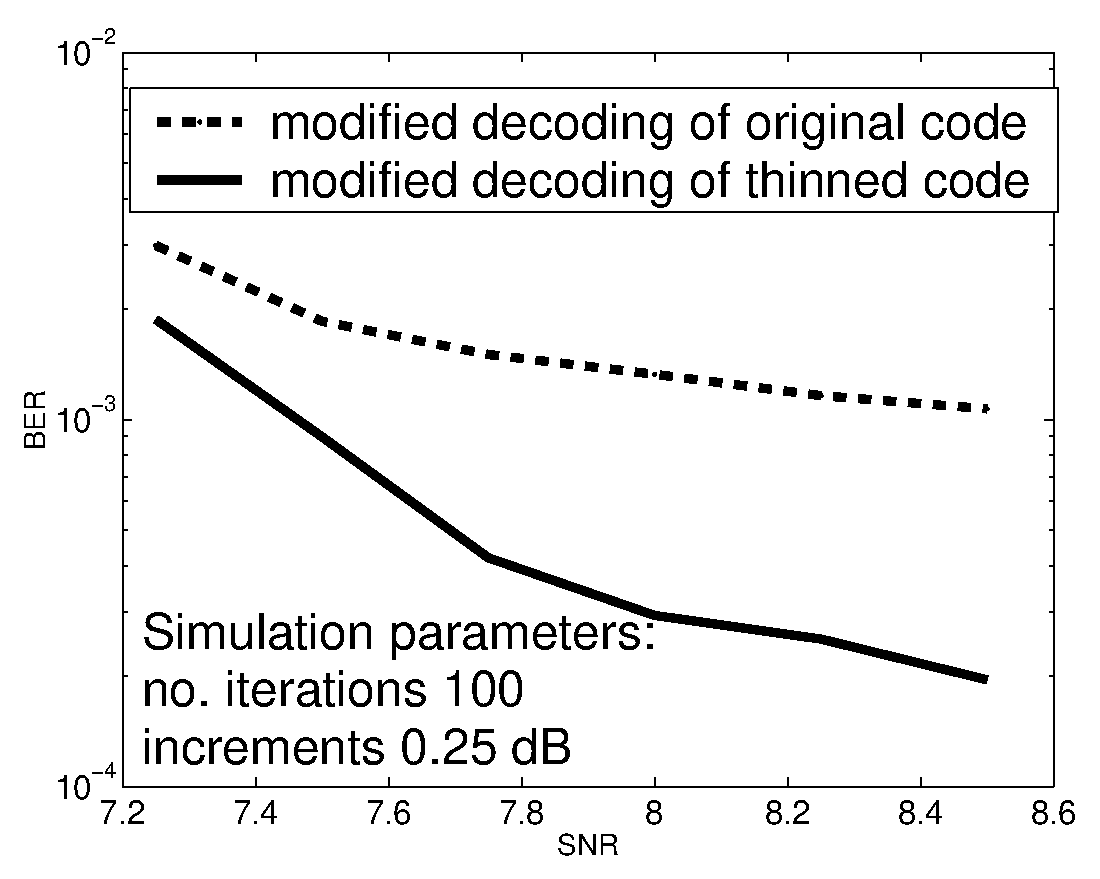
\includegraphics[width=2.5in,height=1.18in]{fig233b.eps}
\caption{Performance of LDPC (529,462) over AWGN with one
repetition} \vspace{-0.05in}
\end{figure}



\section{Concluding remarks}
We proposed a technique for modifying array-based LDPC codes when
varying sampling rate may cause repetition of symbols. Allowing a
small loss in rate, we systematically expurgate the code to get a
thinned code with significantly improved synchronization error
correction properties. We also gave a scheme for constructing
$t$-repetitions correcting families of sequences. Incorporating
multiple synchronization error correction capabilities in
array-based LDPC codes and other codes of interest is a topic for
future research.

% conference papers do not normally have an appendix

% use section* for acknowledgement
\vspace{-0.1in}
\section*{Acknowledgment}
% optional entry into table of contents (if used)
%\addcontentsline{toc}{section}{Acknowledgment}
The authors would like to thank Marvell Semiconductor Inc. and
U.C. MICRO program for supporting their research.



\begin{thebibliography}{17}

%\bibitem{Shannon1948}
%C. E. Shannon, ``A mathematical theory of communication,''
%\emph{Bell Syst.\ Tech.\ J.}, vol.\ 27, pt.~I, pp.~379--423, 1948;
%     pt.~II, pp.~623--656, 1948.
\bibitem{aji}
S. Aji and R. McEliece, ``The generalized distributive law",
\emph{IEEE Trans.  Inform. Theory} vol.\ 46(2), pp.~325--43, March
2000.
%\bibitem{tam}
%P. Bhagawat, M. Uppal and G. Choi, ``FPGA based implementation of
%decoder for array low-density parity check codes,''%In \emph{Proc. of
%\emph{ ICASSP}, 2005, pp.~29--32.%, Philadelphia, PA, USA.
%\bibitem{bours:94}
%P.A.H. Bours, ``Construction of fixed-length insertion/deletion
%correcting runlength-limited codes,'' \emph{IEEE Trans. Inf.
%Theory}, vol.\ 40(6), pp.~1841--1856, Nov. 1994.
\bibitem{cmnv:03}
G. Chen, M. Mitzenmacher, C. Ng and N. Varnica, ``Concatenated
codes for deletion channels,'' \emph{Int. Symp. Inform. Theory},
2003, p.~218.%, Yokohama, Japan.
\bibitem{dmackay:01}
M.C. Davey and D.J.C. MacKay, ``Reliable communication over
channels with insertions, deletions and substitutions,''
\emph{IEEE Trans. Inf. Theory}, vol.\ 47(2), pp.~687--98, Feb.
2001.
\bibitem{techArray:06} L. Dolecek and V. Anantharam, ``On array-based LDPC codes in channels
with varying sampling rate,'' available at
www.eecs.berkeley.edu/\~{}dolecek/papers
\bibitem{techRM:06} L. Dolecek and V. Anantharam, ``Using Reed-Muller codes in channels with synchronization and substitution errors,'' available at www.eecs.berkeley.edu/\~{}dolecek/papers
\bibitem{ibm:02} % linear time encoding    dsl app
E. Eleftheriou and S. \"{O}l\c{c}er, ``Low density parity check
codes for digital subscriber lines,'' \emph{Int. Conf. on Comm.},
2002, pp.~1752--57.
\bibitem{fan}
J. L. Fan, ``Array-codes as low-density parity-check codes,''
\emph{Second Int. Symp. on Turbo Codes and Related Topics}, 2000,
pp.~543--46.
%\bibitem{ferr:97}
%H.C. Ferreira, W.A. Clarke, A.S.J. Helberg, K.A.S. Abdel-Ghaffar and
%A.J. Han Vinck, ``Insertion/deletion correction with spectral
%nulls,'' \emph{IEEE Trans. Inf. Theory}, vol.\ 43(2), pp.~722--732,
%March 1997.
\bibitem{klove:95}
T. Kl{\o}ve, ``Codes correcting a single insertion/deletion of a
zero or a single peak-shift,'' \emph{IEEE Trans. Inf. Theory},
vol.\ 41(1), pp.~279--83, Jan. 1995.
\bibitem{kbek:04}
P. Kovintavewat, J. R. Barry, M. F. Erden and E. Kurtas,
``Per-survivor timing recovery for uncoded partial response
channels,''\emph{Int. Conf. on Comm.}, 2004, pp.~2715--19.%, Paris,
%France.
\bibitem{lev:66}
V. I. Levenshtein, ``Binary codes capable of correcting deletions,
insertions and reversals,'' \emph{Sov. Phys.-Dokl.}, vol.\ 10(8),
pp.~707--10, Feb. 1966.
\bibitem{liu:02}
J. Liu, H. Song and B.V.K.V. Kumar, ``Symbol timing recovery for
low-SNR partial response recording channels,'' \emph{Globecom}
2002, pp. 1129--36.%, San Francisco, CA, USA.
\bibitem{mittel:02}
T. Mittelholzer, ``Efficient encoding and minimum distance bounds
of Reed-Solomon-type array codes,'' \emph{Int. Symp. Inform.
Theory}, 2002, p. 282.%, Lausanne Switzerland.
\bibitem{mcla:02}
A. R. Nayak, J. Barry and S. W. McLaughlin, ``Joint timing
recovery and turbo equalization for coded partial response
channels,'' \emph{IEEE Trans. On Magnetics}, vol.\ 38(5),
pp.~2295--97, Sept. 2002.
\bibitem{sloane:00}
N.J.A. Sloane, ``On single deletion correcting codes,'' 2000.
Available at http://www.research.att.com/\~{ }njas/doc/dijen.pdf
\bibitem{kumar:04} %mr app
H. Song and B.V.K.V. Kumar, ``Low density parity check codes for
partial response channels,'' \emph{IEEE Signal Proc. Magazine},
vol.\ 21(1), pp.~56--66, Jan 2004.
\bibitem{vt:65}
R. R. Varshamov and G.M. Tenengolts, ``Codes which correct single
asymmetric errors,'' \emph{Avtomatika i Telemehkanika}, vol.\
26(2), pp.~288--92,1965.
\bibitem[17]{yanghell:03}
K. Yang and T. Helleseth, ``On the minimum distance of array codes
as LDPC codes," \emph{IEEE Trans. Inf. Theory}, vol.\ 49(12),
pp.~3268--71, Dec. 2003.
\end{thebibliography}

%\include{test}
\include{introb}
\include{iterativeBG}
\include{arrayabs5}
%\chapter[Absorbing Sets of Tanner LDPC Codes]{Absorbing Sets Analysis of Tanner LDPC Codes}

\section{Tanner LDPC Code Construction}

\section{Theoretical Results}\label{theo1}

%\include{is}
\chapter[Conclusion and Future Extensions]{Conclusion and Future Extensions}
\label{ch:conclusion}

% ===============================
% Part III: Back Matters
%           - bibliography
%           - appendix
%           - index
% ===============================

%\ssp
%\bibliographystyle{ieeetr}
\bibliography{refs}
\include{refs}
%\include{append}

\end{document}
